\documentclass[a4paper, 12pt, oneside]{book}
\usepackage[left=1.25in,top=1in,right=1in,bottom=1in]{geometry}
\usepackage[utf8]{inputenc}
\usepackage{booktabs}
\usepackage{tabularx}
\usepackage{multirow}
\usepackage[framemethod=TikZ]{mdframed}
\usepackage{arabluatex}
\usepackage{pifont}
\usepackage{newpxmath} % math font is Palatino compatible
% \usepackage[nomath]{fontspec}
% \usepackage{amsmath}
\usepackage{setspace}
\usepackage[explicit,compact]{titlesec}
\usepackage[hidelinks]{hyperref}
\usepackage{apacite} % load this after hyperref
\setmainfont{TeX Gyre Pagella} 

% remove this if you want to print it as paperback
\setlength\oddsidemargin{\dimexpr(\paperwidth-\textwidth)/2 - 1in\relax}
\setlength\evensidemargin{\oddsidemargin}

% arabluatex options
\SetTranslitConvention{arabica}

% mdframed options
% \definecolor{amethyst}{rgb}{0.6, 0.4, 0.8}
% \mdfdefinestyle{MyFrame}{%
%     linecolor=amethyst,
%     outerlinewidth=0.3pt,
%     roundcorner=3pt}
\newcounter{ortho}[section]\setcounter{ortho}{0}
\renewcommand{\theortho}{\arabic{section}.\arabic{ortho}}
\newenvironment{ortho}[2][]{%
\refstepcounter{ortho}%
\ifstrempty{#1}%
{\mdfsetup{%
frametitle={%
\tikz[baseline=(current bounding box.east),outer sep=0pt]
\node[anchor=east,rectangle,fill=orange!50]
{\strut Orthography~\theortho};}}
}%
{\mdfsetup{%
frametitle={%
\tikz[baseline=(current bounding box.east),outer sep=0pt]
\node[anchor=east,rectangle,fill=orange!50]
{\strut Orthography~\theortho:~#1};}}%
}%
\mdfsetup{innertopmargin=10pt,linecolor=orange!50,%
linewidth=1.5pt,topline=true,roundcorner=3pt,%
frametitleaboveskip=\dimexpr-\ht\strutbox\relax
}
\begin{mdframed}[]\relax%
\label{#2}}{\end{mdframed}}

% for full expanding width table
\newcolumntype{Y}{>{\centering\arraybackslash}X}

\def\title{\Large\bf Text Analytics of the Qur'\=an}
\def\author{Al-Ahmadgaid Bahauddin Asaad}
\def\program{\bf Master of Arts in Islamic Studies}
\def\ddate{May 2025}

\titleformat{\chapter}[block]
    {\vspace{-3cm}\bfseries\Large\centering}{\chaptertitlename}{0.5ex}{\;\bfseries\Large\thechapter\\#1}

\titleformat{name=\chapter,numberless}[block]
    {\vspace{-3cm}\bfseries\Large\centering}{#1}{0.5ex}{}

\titleformat{\section}[block]
    {\bfseries\normalsize}{\thesection}{0.5ex}{\;#1}

\titleformat{\subsection}[block]
    {\bfseries\normalsize}{\thesubsection}{0.5ex}{\;#1}

\begin{document}
\begin{center}
\vspace{-2cm}\title
\end{center}
\addcontentsline{toc}{chapter}{Title Page}
\thispagestyle{empty}
{\baselineskip=1.0\baselineskip
\begin{center}
\vspace{2cm}
by\\
\vspace{3cm}
{\bfseries\author}\\
\vspace{3cm}
{
Submitted to the \textit{Institute of Islamic Studies}\\[0.2cm]
in partial fulfillment of the requirements for the degree of\\[.2cm]}
{\program}\\
\vspace{2.8cm}

\includegraphics[scale=0.08]{uplogo}\\[0.2cm]
{\large \textsc{University of the Philippines}}\\[0.2cm]
Diliman, Quezon City\\
\vspace{3.4cm}
{\ddate }
\end{center}

}
\doublespacing
% \chapter*{Dedication}
\addcontentsline{toc}{chapter}{Dedication}
\begin{center}
    \txarb{إلى الرجل المعروف لدى البعض كمخطط ومتحدث عام، ولكنه معروف لدى الكثيرين كمعلم، ومصمم، ونجار، وسائق دراجة ثلاثية، وصياد سمك، وبشكل خاص أب متواضع، أبانا العزيز، غرواس س. أسعد. نسأل الله أن يمنحك أعلى درجات الجنة، وأن يجمعنا جميعاً هناك. أشتاق إليك كثيراً، شكراً لك على كل شيء.}\\

    \textit{To the man known to some as a planner and a public speaker, but known to many as a teacher, designer, carpenter, tricycle driver, fisherman, and most especially a humble father, our dear papa, Garwas S. Asaad. May Allah \txarb{\fontspec{Scheherazade New} ﷿} bless you with the highest of} \arb{jannaT} \textit{, and may He unite us all there together. I miss you so much pa, magsukul ma kamemon.}\\
    \begin{minipage}{.6\linewidth}
        \centering
        \vspace{4cm}
        \arb[fullvoc]{'afalA yatadabbarUna 'l-qur'Ana walawkAna min `indi.gayri 'l-lahi lawajadUA" fIhi "axtilAfaN ka_tIraN}\\
        \textit{Will they not think about this Qur'an? If it had been from anyone other than God, they would have found much inconsistency in it.}\\
        {\sc Qur'an 4:82}\\[2cm]
        \arb[fullvoc]{wa`ibAdu 'l-ra.hmAni 'lla_dIna yam^sUna `alaY" 'l-'ar.di hawnaN wa-'i_dA xA.tabahumu\\
        'l-j---------------------Ahi---------------------lUna 
        q---------------------Al---------------------UA" sa---------------------lAm---------------------aN}\\
        \textit{The servants of the Lord of Mercy are those who walk humbly on the earth, and who, when aggressive people address them, reply, with words of Peace.}\\
        {\sc Qur'an 25:63}\\[1cm]
    \end{minipage}
\end{center}
% \chapter*{Acknowledgement}
\addcontentsline{toc}{chapter}{Acknowledgement}
{\centering

\includegraphics[scale = 1]{img/bismillah.jpg}\\[-.3cm]
(In the name of Allah, the Entirely Merciful, the Especially Merciful)\\[3cm]
}
\textit{The author would like to acknowledge his thesis adviser, Prof. Julkipli M. Wadi, for his patience and guidance; his thesis panels, Dr. Joselito C. Magadia (UPD School of Statistics), for his valuable insights on the theory, algorithm, and modeling aspect of the paper. Lastly, the author would like to acknowledge his family, friends, co-workers, and his chuchay for their moral support.}\\[2cm]
\begin{center}
    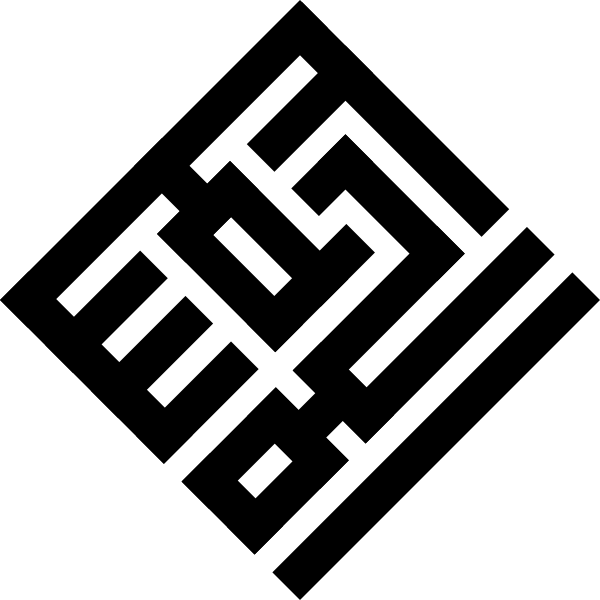
\includegraphics[width=0.1\textwidth]{img/alasaad-logo.png}\\
    Al Asaad\\
    \url{https://al-asaad.com}\\[-0.3cm]
    \url{https://al-asaad.vercel.app}
\end{center}
\chapter*{Abstract}
\addcontentsline{toc}{chapter}{Abstract}
This thesis presents a novel application of Statistics and Machine Learning techniques to analyze the Qur'\=an, complementing traditional methodologies while approaching the sacred text with appropriate respect and care. The research examines structural and linguistic patterns through multiple analytical lenses. Descriptive statistics reveal distinct clusters between \arb[trans]{makkiyyaT} \arb{makkiyyaT} and \arb[trans]{madaniyyaT} \arb{madaniyyaT} \arb[trans]{suwar} \arb{suwar}, with the latter demonstrating higher median values and greater variability. Morphological analysis of the root word \arb[trans]{Alh} \arb[novoc]{Alh} shows its common form \arb[trans]{'l-lahi} \arb[fullvoc]{'l-lahi} predominantly appears in \arb[trans]{madaniyyaT} \arb{madaniyyaT} chapters, while rarer forms (\arb[trans]{--|"'Alihati} \arb[fullvoc]{--|"'Alihati} and \arb[trans]{'alihatu} \arb[fullvoc]{'alihatu}) are exclusive to \arb[trans]{makkiyyaT} \arb{makkiyyaT} texts. Examination of manuscripts from 660-1000 CE from the Corpus Coranicum project confirms the preservation of these morphological patterns, supporting the integrity of oral transmission. For rhythmic analysis, the paper propose visualization techniques including line plots, heatmaps, rhythmic graphs, and histogram density plots, revealing strong patterns where approximately 70\% of \arb[trans]{'ayaT} \arb{'ayaT} endings feature transitions from short to long vowels. The paper further investigate concentric structures in \arb[trans]{sUraTu 'l-baqara} \arb{sUraTu 'l-baqara} using a novel Genetic Algorithm approach to objectively identify structural borders, employing CL-AraBERT for word embeddings with Cosine Distance metrics. The resulting optimal structural borders ($A$, $B$, $C$, $D$, $C^*$, $B^*$, $A^*$) were thematically analyzed using GPT-4o, confirming the concentric arrangement. This research demonstrates the value of computational methods, particularly the Julia programming language with libraries like QuranTree.jl and Yunir.jl, in revealing new insights into this complex, multi-layered text while respecting its sanctity and significance.

\chapter{Introduction}
\label{ch:introduction}
The use of scientific computing to studying the Qur'\=an is still in its early stage in the fields of Islamic Studies and Statistical and Machine Learning applications. This study will indeed benefit not only researchers from Islamic Studies but also Statisticians and Machine Learning researchers who are into text analytics. Having said that, it is therefore necessary to provide context to audiences of these disciplines to provide background on the state of Qur'\=anic studies and the increasing adoption of scientific methodology to studying humanities.
\section{Background}
The Qur'\=an or \arb[trans]{al-qur'An} \arb{al-qur'An} meaning \textit{the recitation}, the holy book of Islam, is revered by 1.9 billion (according to 2020 projection of \shortciteA[p.~13]{pewresearch}) Muslims across the globe as the literal words of God. Muslims believed that the Qur'\=an was gradually revealed (Qur'\=an 25:32) to Prophet Muhammad \arb{\arbmark{slm}} through angel \arb[trans]{jibrIl} \arb{jibrIl} or Gabriel (Qur'\=an 2:97). The Qur'\=an contains 77,429 Arabic words in total, which covers only 56 percent of the Greek New Testament which has 138,020 words in total \cite[p.~11]{sinai2017}. 

The Qur'\=an is divided into \textit{s\=urahs} \arb{sUr} which are the equivalent of chapters, each containing \arb[trans]{'ayAt} \arb{'ayAt} (meaning \textit{signs}), which are the equivalent of verses. The \textit{s\=urahs} \arb{sUr} are not arranged in chronological order as in the Bible's books and chapters, but rather arranged in monotonically decreasing length of number of verses after the first \textit{s\=urah} \arb{sUraT} (\textit{see} Figure \ref{fig:ayah_word_count}). The \textit{s\=urah} \arb{sUraT} of the Qur'\=an can be categorized into two types: the \arb[trans]{makkiyyaT} \arb{makkiyyaT} (Meccan) and \arb[trans]{madaniyyaT} \arb{madaniyyaT} (Medinan). The categories refer to the geographical location of where the \textit{s\=urah} \arb{sUraT} was revealed. Figure \ref{fig:ayah_word_count} shows the grouping of the \textit{s\=urahs} \arb{sUr}. Note that some of the \textit{s\=urahs} \arb{sUr} have mixed geographical locations\footnote{\textit{see} list of the location in \url{https://tanzil.net/docs/revelation_order}}, that is, a few of the \arb[trans]{'ayAt} \arb{'ayAt} in it were revealed in other geographical location apart from the geographical location of the rest of the \arb[trans]{'ayAt} \arb{'ayAt}. Therefore, the categorization in Figure \ref{fig:ayah_word_count} highlights the geographical location of the majority of the \arb[trans]{'ayAt} \arb{'ayAt} in the \textit{s\=urah} \arb{sUraT}.

\begin{figure}[!b]
    \centering
    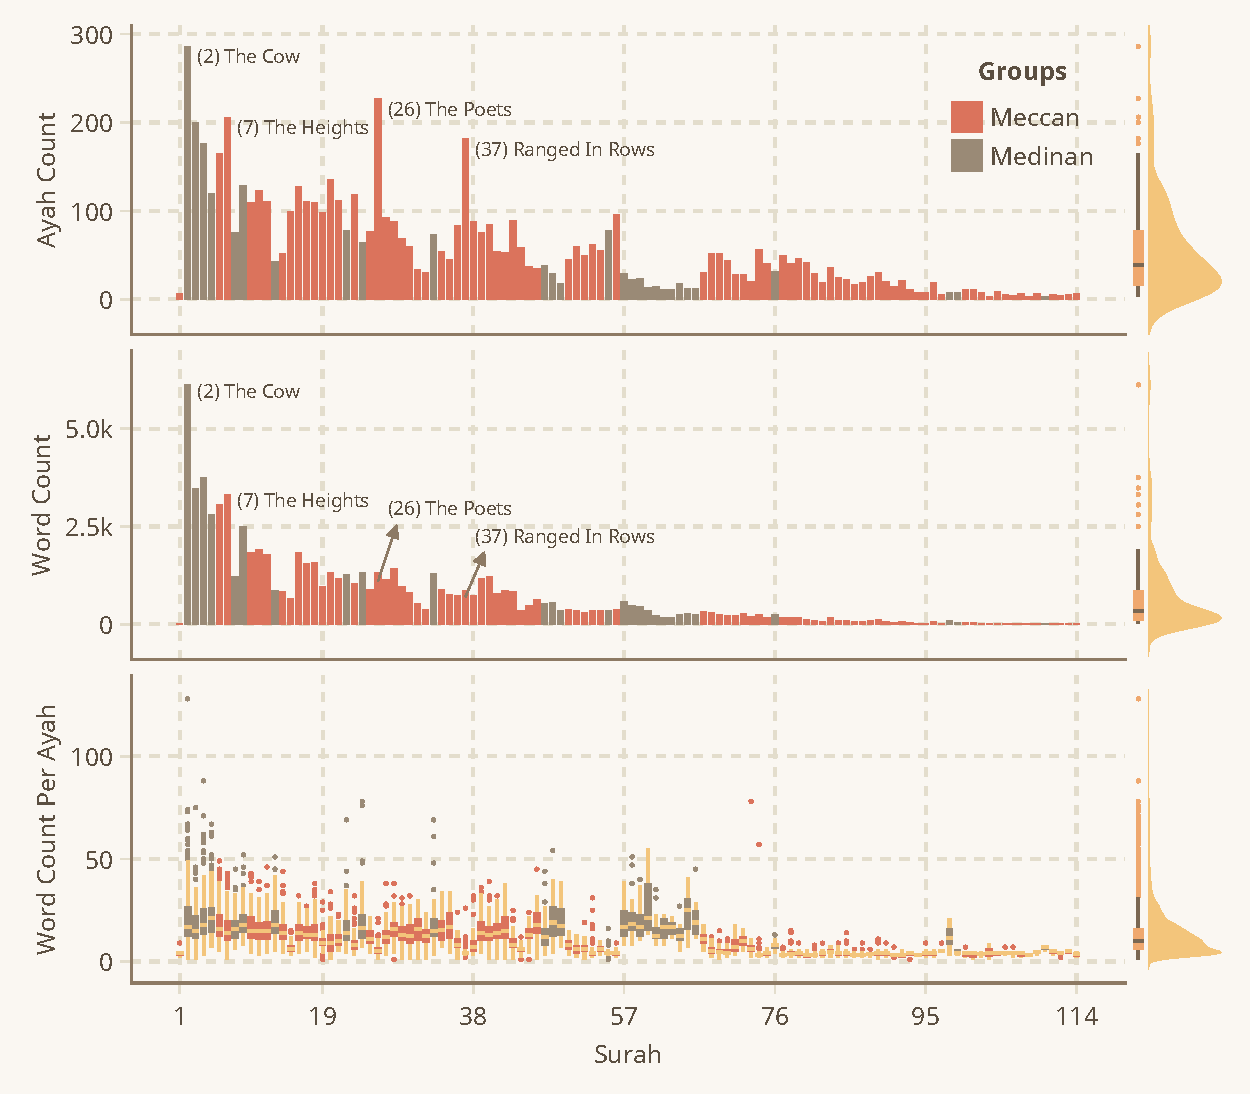
\includegraphics[width=\textwidth]{img/plot1.pdf}
    \caption{Statistics of the words and \arb[trans]{ayAt} \arb{ayAt} (verses) of the Qur'\=an}
    \label{fig:ayah_word_count}
\end{figure}

The Qur'\=an (meaning \textit{the recitation}) was revealed \textit{orally} by angel \arb[trans]{jibrIl} \arb{jibrIl} to Prophet Muhammad \arb{\arbmark{slm}} and passed onto other believers through oral tradition (reciting the Qur'\=an to students repeatedly so as to memorize it, instead of writing it down and let the believers read it and memorize it). Memorizing 77,429 Arabic words of the Qur'\=an through oral transmission can be a difficult task, but what aids this memorization is the rhythm feature of the Qur'\=an. According to one Orientalist, \citeA{sinai2017}, "rhyme, however, or rather a periodically recurrent word-final assonance, is a feature of the Qur'\=an throughout, and it naturally partitions the \textit{s\=urah} \arb{sUraT}." Indeed, because of this feature, it makes it easy to memorize the entire Qur'\=an, and the one who do so is called \arb[trans]{hafi.z} \arb{hafi.z} meaning \textit{one who remembers} or \textit{keeper}. Qur'\=an memorization contest is a common event in Muslim countries, the Philippine embassy has hosted one in 2022 in Saudi Arabia \cite{mb2022}.

According to the Muslim tradition, the oral transmission of passing the Qur'\=an from a \arb[trans]{hafi.z} \arb{hafi.z} to new believers was gradually put into writings as requested by the believers themselves. The idea was brought up after the battle of Yamama, where many of the Muslims who died were \arb[trans]{qurrA'} \arb{qurrA'} (\textit{the one who properly recite the Qur'\=an}), and so fearing that their numbers will reduce in other battle fields, Umar ibn al-Khattab \arb{`umaru bnu 'l-xa.t.tAb} (who became the second caliph) suggested to the first caliph, Ab\=u Bakr 'Abd All\=ah ibn 'Ab\=i ibn 'Ab\=i Qu\d{h}\=afa, \arb{'abU bakriN `abdu 'l-lAhi 'ibni 'abiY qu.hAfaTa} or short for Ab\=u Bakr \arb{'abU bakr}, to collect the Qur'\=an into writing. Ab\=u Bakr then authorized Zaid ibn Thabit \arb{zaydi bni _tAbitiN} for the task. According to Zaid, he started collecting from the leafless stalks of the date-palm tree and from the pieces of leather and hides and from the stones, and from the chests of men (who had memorized the Qur'\=an, i.e. the \arb[trans]{hafi.z} \arb{hafi.z})\footnote{\textit{see} \url{https://sunnah.com/bukhari:7191}}. Long story short, the effort was finally codified by the third caliph, Uthman ibn Affan \arb{`u_tmAnu bnu `affAn} in the year 645 CE, which was then recopied and distributed to the different regional capitals of the early Islamic empire of that time. The rest of the copies outside this codification were then burned\footnote{\textit{see} \url{https://sunnah.com/bukhari:4987}} down in order to have one standard Qur'\=an. The Qur'\=an nowadays is therefore assumed to be based on Uthmanic codex because of the story mentioned. That is, if indeed Uthman has ordered to burn other copies of the Qur'\=an outside his codification, then what's left should only be based on his codex or archetype, and that should only be the inherited codex of the Muslims today.

The Qur'\=an is believed by the Muslims to have been preserved since it was first recited by angel \arb[trans]{jibrIl} \arb{jibrIl} or Gabriel to the Prophet \arb{\arbmark{slm}}. Many orientalists had been skeptic about this claim, for example, John Wansbrough theorized that the Qur'\=an was collected over a 200-year period \cite<\textit{see}>[p.~101]{wansbrough2004} after the death of the Prophet \arb{\arbmark{slm}}, instead of within a few years after the death of the Prophet \arb{\arbmark{slm}}. However, recent findings through radiocarbon dating brings forward strong evidence of potential preservation of the whole Qur'\=an, which the Muslims believed to be so. For example, the Birmingham Qur'\=an manuscript discovered in 2015 is dated to be between 568 and 645 CE with 94.5\% accuracy, making it among the oldest Qur'\=anic manuscript in the world \cite<\textit{see} >{bu2015}. Its predicted range of years intersects with the lifetime (570 to 632 CE) of the Prophet \arb{\arbmark{slm}}. What is interesting is that the Birmingham Qur'\=an is consistent with the Qur'\=an today, word-by-word and letter-by-letter\footnote{The orthography of the Arabic letters in the early days had no diacritics and were written in its basic consonantal skeleton. That is, Arabic orthography and grammar were in their nascent when the Qur'\=an was revealed, and therefore has to adjust and catch up, to capture and preserve the proper recitation of the Qur’an.}, see Figure \ref{fig:birmingham}. This is indeed another evidence that the Qur'\=an today was codified by Uthman since the discovery of the Birmingham Qur'\=an manuscripts have confirm it. In addition to this, the Sana'a Palimphest is also among the oldest Qur'\=an radiocarbon dated to be between 578 CE and 669 CE with 95\% accuracy \cite{behnam2010}, which according to \citeA{sinai2017}, "neither does the edited portion of the Sana'a palimpsest offer evidence for additional or missing verses or for a divergent verse order within the \textit{s\=urahs} \arb{sUr}." Given these discoveries on the recent Quranic manuscripts, the claim of \citeA[p.~101]{wansbrough2004} is now untenable \cite<\textit{see}>{sinai_2014}.

\begin{figure}[!b]
    \centering
    \includegraphics[width=\textwidth]{img/birmingham.jpg}
    \caption{20th Century Qur'\=an (left) in its fully featured orthographies vs Birmingham Qur'\=an dated between 568 and 645 CE (right) in its basic consonantal skeleton. Image from \protect\citeA{wikibirmingham}.}
    \label{fig:birmingham}
\end{figure}

One likely reason as to why the scribes were able to preserve the Qur'\=an in the two folios of the Birmingham Qur'\=an manuscripts follows from the fact that the Qur'\=an is firstly memorized before it was decided to be written. So that, the \mbox{Topkapi} manuscripts that contain 99\% (only 23 verses missing)---dated around 701 to 750 CE \cite{karatay1962}\footnote{\textit{see also} \url{https://corpuscoranicum.de/en/manuscripts/1977/page/1-410?sura=1&verse=1}}, that is, around 69 to 118 years after the death of the Prophet \arb{\arbmark{slm}}---of the Qur'\=an today was likely partly written from memory. This is possible since the Qur'\=an possesses a rhytmic feature (that aids with memorization) that naturally divides its verses or \arb[trans]{'ayAt} \arb{'ayAt}, and that the Qur'\=an memorization competition is still held to this day \cite<as in the example of >{mb2022}, apart from the fact that it needs to be recited (any chapter after the first chapter of the Qur'\=an according to the choice of the worshipper) every prayer from memory. Bottomline, there are many avenues for Qur'\=an recitation from memory, and these have helped in its preservation. Moreover, since there are no significant evidence of insertion or malicious intention on addition or revision in all of the extant Qur'\=anic manuscripts so far, some Orientalists came up with other theories of insertions on the basis of the literary style of the Qur'\=an, see for example \citeA[p.~92]{sinai2017}, where verse 102 of \arb[trans]{sUraT 'l-.sAffAt} \arb{sUraT 'l-.sAffAt} or The Chapter of \textit{Ranged in Rows} is theorized as addition because it is longer compared to other verses in the said chapter, refer to \citeA[p.~92]{sinai2017} for his other reasonings. Nonetheless, the Qur'\=an is indeed stable based on the extant manuscripts.

Furthermore, the vastness of the early Islamic empire meant that different Muslim regional capitals have covered populations with different Arabic dialects, and so to accommodate these differences, Muslims believed that there were seven variant readings of the Uthmanic codex. Variant readings are defined as different pronunciations of the same word, in this case seven Uthamnic Qur'\=an for seven different pronunciations. The \arb[trans]{.hadI_t} \arb{.hadI_t} or \textit{narration} comes from Ubayy ibn Ka'b \arb{'ubayyi bin ka`b} who reported\footnote{source: \url{https://sunnah.com/muslim:821a}} that the Prophet \arb{\arbmark{slm}} was near the tank of Banu Ghifar that \arb[trans]{jibrIl} \arb{jibrIl} or Gabriel came to him and said: "... Allah has commanded you to recite the Qur'\=an to your people in \textit{seven dialects}, and in whichever dialect they would recite, they would be right." Recent work of \citeA{sidky2020} shows that the material evidence on the regional variants is in remarkable agreement with well-attested written variants documented in the traditional Muslim literature.

Muslim and non-Muslim scholars alike have been extremely interested in understanding the unique literary characteristics of the Qur'\=an. As mentioned earlier, unlike other books like the Bible (arranged in chronological order), the Qur'\=an does not follow any obvious organization. In addition to this, a \textit{s\=urah} \arb{sUraT} does not fit the exact definition of a chapter. Indeed, the name attached to a \textit{s\=urah} \arb{sUraT} is often decided as the unique entity mentioned in the said \textit{s\=urah} \arb{sUraT}, its main purpose is to help early Muslims distinguish which \textit{s\=urah} \arb{sUraT} they are talking about, this is contrary to the chapter name where the associated name is obviously the main topic of the chapter. Further, as described by \citeA{sinai2017}, "... the compositional unity of the long surahs located at the beginning of the corpus is anything but obvious: at least at first sight, they can appear a flit back and forth between different topics in a largely haphazard manner. This impression is not limited to Western readers: even pre-modern Muslim scholars have often approached their scripture as a quarry of unconnected verses and groups of verses that bear little intrinsic relation to what precedes and follows." It wasn't until \citeA{Neuwirth_2007}, that the compositional unity of the Qur'\=an can be observed in tighter literary unities, as \citeA{Neuwirth_2007} showed that the many of these texts display a tripartite structure and are often constructive around a narrative middle part \cite{sinai2017}. Samples of the organizational style of the Qur'\=an was shown in \citeA[p.~88]{sinai2017}.

\section{Rationale of the Study}\label{sec:rationale}
Attempts at understanding the Qur'\=an by Qur'\=anic scholars were mostly done with the use of manual processes, that is, studying the scriptures by going through its content one-at-a-time manually. However, with the advent of computers, some researchers have started using it to aid in their study. The first known to have used computers for studying the Qur'\=an was likely Rashad Khalifa in 1968\footnote{\textit{see} \url{https://www.masjidtucson.org/quran/miracle/a_profound_miracle_sura68nun133.html}}, where he studied the significance of the mysterious initials at the beginning of some \textit{s\=urahs} \arb{sUr}. Rashad uploaded the Qur'\=an into his computer by transliterating the Arabic letters and other Qur'\=anic orthographies into Roman letters and symbols that the computer can easily parse. This approach of using computers to find new insights is more common in the field of science, and it was new to the field of Qur'\=anic studies.

Indeed, to proceed with the use of scientific computing, the Qur'\=an will be treated as the data that needs to be analyzed using what is called Natural Language Processing (NLP), a branch of Machine Learning (ML) that aims to understand natural languages, such as Arabic. To instruct the computer to do Statistical analyses, ML, or NLP, one needs to use a \textit{software application} or a formal language called \textit{programming language}. There are several programming languages that the computer can understand. The popular one for researchers in the field of sciences are Python, R, and sometimes Julia \shortcite{Julia2017}. These programming languages will be used to construct instructions for computer. Therefore, if the data is the Qur'\=an, then there should be a way to interface with it using any of these programming languages. Or alternatively, there should be a way to upload it into the chosen programming language and encode the Arabic letters into something that can be easily parsed by the computer, like what Rashad \mbox{Khalifa} did. Having said that, there are indeed some programming languages with libraries or packages for interfacing with the Qur'\=an, and this is true for Python, R, and \mbox{Julia}. For this study, Julia programming language since its  library for interfacing the Qur'\=an using the QuranTree.jl\footnote{\textit{see} \url{https://alstat.github.io/QuranTree.jl/stable/}} has more features compared to those available in R and Python \cite<\textit{see}>{asaad2021qurantree}. QuranTree.jl is based on Tanzil\footnote{\url{https://tanzil.net/download/}} for the Qur'\=anic Arabic texts, and \citeA{dukes-habash-2010-morphological} for morphological annotation, which both libraries from R and Python do not have in terms of morphological annotation from \citeA{dukes-habash-2010-morphological}.

Now that the programming language for this paper is identified, next is to understand how Statistics and Machine Learning can help in studying the Qur'\=an. Statistics is a branch of Science that aims to study features or characteristics of data generated from a random phenomenon. The findings of Statistical analyses can then be used to make conclusions or predictions of the general population of the data or general characteristics of the data. Machine Learning or ML, on the other hand, is a branch of Artificial Intelligence that heavily intersects with Statistics, albeit with distinct differences as well. Both Statistics and ML aims to characterize data by learning its features, but ML research aims on complex models that are often inspired by simpler models from Statistics. Therefore, one can think of Statistics as one of the fundamentals of ML. 

One of the goals of Statistics and Machine Learning is to summarize all of the learned features into a hypothesized equation or hypothesized mathematical formula whose parameters or weights are optimized to capture the most characteristics of the data. It is called hypothesized equation since the researcher is the one who decide which family of equation best describe the characteristics of the data. The said equation is called a \textit{model}. Therefore, a model is a generic entity that can be fitted or molded to capture the features of the data. Mathematically and in general, a model can be written as:
\begin{equation}\label{eq:general_model}
    \hat{y}:=h(x|\mathbf{\theta}),
\end{equation}
which is a mapping between the sets $\mathcal{X}$ and $\mathcal{Y}$ where $x\in\mathcal{X}$ and $y\in\mathcal{Y}$ through a hypothesized function $h$. The idea of modeling is to find the optimal value of $\mathbf{\theta}$ in such a way it will minimize the error between the actual data (represented by $y$ below) and the predicted one $\hat{y}$:
\begin{equation}
    \varepsilon:=y-\hat{y}=y-h(x|\mathbf{\theta}).
\end{equation}

To help understand the concept of modeling, and relate it to the fashion industry, which the author assumes most readers are familiar with, a model in a fashion industry is responsible for representing the characteristics of the target customers (in Eq. \ref{eq:general_model} this is $y$). Therefore, for a clothing company, they hire Asian models (in Eq. \ref{eq:general_model}, this is $\hat{y}$ or $h(x|\mathbf{\theta})$) to target Asian customers (in Eq. \ref{eq:general_model} this is $y$). So that, when these models wore the clothes sold by the said company, the potential customer will more or less be able to relate to the model, and be able to imagine themselves wearing that same clothes as well, which help them incline to buying the said clothing. The model, therefore, does not necessarily have the looks of every target Asian customers, but at least in terms of height, skin tone, hair, and other common Asian features, the model will likely have it, or at least the difference is more or less minimal (in Eq. \ref{eq:general_model}, the difference is represented by $\varepsilon:=y-\hat{y}$). The question now is, what are the benefits that this model can bring to the clothing company? Well, the clothing company will be able to create products that are tailored to their Asian customers using the said model, since the company will have the right baseline measurements needed. Relating this analogy to the technical concept discussed earlier, you can think of the target customers as the
real or actual data (in Eq. \ref{eq:general_model} this is $y$), and the model as the same technical term use in Machine Learning and Statistics (in Eq. \ref{eq:general_model} this is $h(x|\mathbf{\theta})$), but this time this technical model is expected to capture the characteristics of the real data analogous to fashion model that is expected to capture the characteristics of the target customer. This Statistical or Machine Learning model brings the following benefit: researchers will be able to study the real data by simply using the model to answer questions that are not available in the sampled real data.

In this paper, the aim is to make use of the Statistical or Machine Learning modeling to understand the characteristics of the Qur'\=an in terms of the morphologies of its canonical text in its modern orthography. More specifically, the following are the general objectives:

\section{Objectives}\label{sec:objectives}
The following are the general and specific objectives of this paper:
\begin{enumerate}
    \item What are the structural characteristics of the Qur'an that can be extracted from its rich morphologies using statistical and large language models?
    \begin{enumerate}
        \item What are the statistics of the Qur'\=an's morphological features in terms of its parts of speech and selected entities like God's name and the prophets names mentioned?
        
        \item How do the rhythmic signatures of the Qur'\=an of the verses looks like and what are statistical insights that can be extracted?
        
        \item What are the supporting statistical insights on the current divisions of the Qur'\=an's verses? 
    \end{enumerate}
    
    \item What other insights that can be extracted from the semantics of the Qur'an's texts using statistical and large language models?
    \begin{enumerate}
        \item How does the theory of \textit{concentrism} be formulated statistically, and what are the insights from the statistical and large language models on this? 
        
        \item How do the surahs are organized in terms of the topics? What are the themes that can be extracted for each of the surahs?
        
        \item How do these extracted themes compare to the summaries of Abdel\linebreak Haleem's English translation of the Qur'an?
    \end{enumerate}
    
    \item How does this combination of statistical, machine learning, and artificial intelligence with the Muslim's traditional literatures help in understanding the Qur'\=an, especially with the advent of Generative AI?
\end{enumerate}

\section{Significance of the Study}\label{sec:significance}
While the Qur'\=an has been extensively studied by Muslims and non-Muslims scholars alike, especially in the topic of Meccan and Medinan surahs, there is still a lot to uncover from the perspective of Computational Statistics. Hence, the significance of this study is that it brings forward new ways of extracting insights from the Qur'\=an by leveraging Computations, Statistics, Machine Learning, and AI, that is still in its early stage in the field of Qur'\=anic Studies. Therefore, this new perspective or process of studying the scripture not only aids the scholars of the Islamic Studies, but may also contribute indirectly to community development and policy makers who use Qur'\=an as part of their decision making.
\section{Scope of the Study}
The paper will cover all chapters of the Qur'\=an both for the Morphological and Topic Modeling analyses, but it will only present the results of \textit{s\=urahs} \arb{sUr} with at least 1000 words. The rest of the result will be part of the web application that can be used to query the Qur'\=an. It will also not delve into the \textit{tafsir} \arb{tafsIr} of each of the verses, but only when necessary for further context.
\section{Thesis Organization}
The paper is organized as follows: Chapter 2 will discuss the related literatures, Chapter 3 will discuss the methodology, Chapter 4 will present the results and discussions, and finally Chapter 5 will contain the conclusion and recommendation. The references and appendices are placed after the Chapter 5.
\chapter{Review of Related Literature}\label{ch:rrl}

As mentioned in the previous chapter, the earliest paper on Qur'\=anic studies using computer was likely the work of Rashad Khalifa in 1968\footnote{\url{https://www.masjidtucson.org/quran/miracle/a_profound_miracle_sura68nun133.html}}, which led to one of his book entitled `The Computer Speaks: God's Message to the World' (\textit{see} \citeA{rashad1981}). While the work of Rashad started at studying the mystery letters in the beginning of some \textit{s\=urahs} \arb{sUr} (for example Qur'\=an 2:1, 3:1, 7:1, etc.), it quickly went on to cover what he calls other \textit{mathematical miracles}, all of which are covered in \citeA{rashad1981}. His work were mainly based on counting the positional statistics of selected entities like names of God relative to other names or words in the Qur'\=an, and showing through counting and simple math of factoring some totals, he showed an interesting matches among these statistics. He was able to do this by transliterating the Qur'\=an into Alpha-Numeric typesets for easy parsing of the computers back then. His findings led him to generalize the claim that God revealed His words through this "mathematical" patterns throughout the Qur'\=an, and that those verses that were off and did not conform to this discovered "mathematical" patterns led him to extensive investigation of the said verses, and concluded that those could be or surely be an insertion that should not have been in the Qur'\=an in the first place. There are two verses that were off according to Rashad, and he called these verses as \textit{false verses}\footnote{\url{https://submission.org/App24.html}}, these are the last two \arb[trans]{'AyAt} \arb{'AyAt} of \arb[trans]{sUraTu 'l-tAwbaT} \arb{sUraTu 'l-tAwbaT} or The Chapter of \textit{Repentance}. These two verses were removed in Rashad's Qur'\=an translation\footnote{\url{https://www.masjidtucson.org/quran/frames/}}. Rashad believed so much on his findings that he self-proclaimed himself to be a messenger\footnote{\url{https://www.masjidtucson.org/submission/faq/rashad_khalifa_summary.html}} with this new findings and that the Qur'\=an nowadays should conform to his found "mathematical" patterns. This self-proclamation led to his assassination.

What the above tells us is that early on with the advent of computers, there was already interest in trying to understand the structural characteristics of the Qur'\=an. This is because the Qur'\=an is not like the Bible that is arranged chronologically, but rather arranged in generally decreasing number of \arb[trans]{'AyAt} \arb{'AyAt} per \arb[trans]{sUraT} \arb{sUraT} as shown in Figure \ref{fig:ayah_word_count}. This unique structure led to different literatures on understanding the Qur'\=an's design in terms of its unique presentation of topics, not only from the Islamic studies researchers but also computer scientists who were into Arabic Natural Language Processing studies. 

Among the pioneers in computational applications for the Qur'\=an is the work of \shortciteA{thabet2004}, who built a stemmer system for the Qur'\=an. A stemmer system is a system for trimming inflected words into its basic form, which grammatically mean its the root form. For example, in English language the root word for \textit{computational}, \textit{computer}, \textit{computation}, and \textit{computerize} is \textit{compute}. Therefore, the root of a word forms different \textit{stems} representing the different words. Hence, the idea of stemming is to trim these words into its basic form, so that it would be easy to do word clustering or grouping through word similarity. According to \citeA{thabet2004}, the rich morphology of the Qur'\=anic language or the Classical Arabic makes it even more difficult to do word stemming. Moving on, \citeA{thabet2005} builds on top of this stemming system, and used it for tokenization of the Qur'\=anic words, and building a statistical methodology for clustering or grouping the chapters of the Qur'\=an, in particular \citeA{thabet2005} used a Agglomerative Hierarchical Clustering based on the Euclidean distance of the adjusted word frequency of a \arb[trans]{sUraT} \arb{sUraT}.

The work of \citeA{thabet2004} and \citeA{thabet2005} used a Qur'\=an's corpus that was transliterated to Roman letters and symbols. Indeed, with the growing interests on studying the Qur'\=an from the lense of Data Analysis and Natural Language Processing, resulted into creating digital corpi of the Qur'\=an that captures the different aspects of its linguistic styles. Hence, a series of work by Sharaf and Atwell led to the following publications: \shortciteA{sharaf2009} studied knowledge representation of the Qur'\=an's verb valences using FrameNet frames, the output of which is a lexical database as a corpus of Qur'\=an's verbs. Further, the work of \shortciteA{sharaf2012} came up with corpus for the annotations of the Qur'\=anic pronouns, the authors named it as QurAna. Building on this work, \shortciteA{sharaf2012b} came up with a corpus for studying Qur'\=anic relatedness based on the commentary of Ibn Kathir \arb{ibn ka_tir}, the authors named this corpus as QurSim. Apart from Sharaf and Atwell, Dukes and Habash was also working on this, but specifically on the morphological annotations. The final and verified\footnote{The authors used online community collaboration for checking or verification of the morphological annotations. This was necessary since the Qur'\=an is a highly regarded book by Muslims, and there should be no mistakes in annotations.} work of the authors is the \shortciteA{dukes-habash-2010-morphological}, which also led to other publications \shortcite{dukes2010online, dukes2013supervised, dukes2010dependency} related to this.

With the establishment of a morphological annotated corpus for the Qur'\=an, the hoped was to have further analyses on the said scripture using statistical and machine learning methodologies. As such, the work of \shortciteA{dukes-habash-2011-one, dukes2015statistical} were among the first to do so, where they constructed a statistical parser through machine learning. This was then followed by \shortcite{siddiqui2013} who used the said corpus for topic modeling using Latent Dirichlet Allocation, the said study started with 114 \arb[trans]{sUwar} \arb{sUwar}, but after processing it went down to 24 \arb[trans]{sUwar} \arb{sUwar} after considering \arb[trans]{sUwar} \arb{sUwar} with 1000 or more words. This was mainly due to the very sparse document term matrix for the Term Frequency - Inverse Document Frequency\footnote{\textit{See} Section \ref{sec:tf-idf}} (TF-IDF) embedding if considering all of the 114 \arb[trans]{sUwar} \arb{sUwar}. Aside from this, the rest have used the corpus by \shortciteA{dukes-habash-2010-morphological} as part of benchmark for morphological analysis or for new lexicographic database, for example \shortciteA{sabtan2017morphological, jarrar-hammouda-2024-qabas-open}.

For the case of \textit{rhythmic analysis} of the Qur'\=an, most of the literatures have looked into the recitation of this rhythmic feature of the Qur'\=an, for example the work of \shortciteA{shekha2013effects, samhani2022rhythms, abdullah2011effect} and \shortciteA{naqvi2020effect} have all investigated the effect of listening to the Qur'\=an recitation on temporal Electroencephalogram (EEG) signals and on human physiology through Electrocardiogram (ECG) signal. The work of \shortciteA{shekha2013effects} subjected 11 students to listen to soft music, hard music, and Qur'\=anic recitation and collected the \textit{alpha} wave signals of it in EEG. The authors used t-test and ANOVA to compare the results from the three input audio. Their findings suggest that the Qur'\=an recitation both during opened eyes or closed eyes while listening to the Qur'\=an have significant magnitude in \textit{alpha} waves electrode. The same study was also conducted by \shortciteA{samhani2022rhythms}, but this time listening to Arab News; Qur'\=anic recitation of \arb[trans]{sUraTu 'l-fAti.haT} \arb{sUraTu 'l-fAti.haT}; and simply resting, that is not listening to any audio. The authors used Analysis of Variance (ANOVA) and Hierarchical Clustering for the resulting Beta oscillation data. Their study found that the said Beta rhythms synchronization
of listening to \arb[trans]{sUraTu 'l-fAti.haT} \arb{sUraTu 'l-fAti.haT} is associated with verbal fluency, academic performance, social
interaction, inhibitory function, movement planning, self-motivation, self-management and
reactivation of sensory features of memory trace as highly activated cluster, followed by working memory, language processing and decision making as medially activated cluster. Another similar study was also done by \shortciteA{abdullah2011effect} with same pattern of output, and that is a good effect on the EEG of the patients. On the other hand, the work of \shortciteA{naqvi2020effect} investigated the effect of the Qur'\=an on the ECG. The authors used different classification models for classifying signals from the Qur'\=an listening. 

While the rhythmic feature is the most obvious feature of the Qur'\=an, the structural arrangement of the topics and verses are not as obvious as compared to any other books. Hence, there have been several attempts to understand these arrangements even from the pre-modern day Muslim scholars. The Basran writer al-Jahiz (d. 255/868 or 869) produced a work entitled \textit{The Composition of the Qur'an}, even a scholar named Abu Bakr al-Nisaburi from 4 AH/10 CE would ask such questions as, "Why is this verse next to the other one?" and, "What is the widom in the plcement of this chapter next to this other one?" \shortcite{farrin2014structure}. According to \shortciteA{farrin2014structure}, since the 1980s, numerous scholars in the field have followed their lead and have begun to show clearly that individual chapters, both short and long, are indeed characterized by a high degree of unity. With that said, among the structure that was found is the \textit{theory of concentrism}, which accordingly is the structural pattern of the Qur'\=an. This was the proposition of Michael Cuypers\footnote{All of his work are written in French. Please refer to \shortciteA{farrin2014structure} for the list of articles written by Cuypers.}. As far as the knowledge of the author, the most comprehensive exposition of the theory of \textit{concentrism} in English is the work of \shortciteA{farrin2014structure}. However, not a single paper have been written for a mathematical formulation of this that can be used for statistical analyses. 

Finally, the recent advancement of large language models (LLM) and its use for the retrieving information resulted into what is called the Retrieval-Augmented Generation (RAG) proposed by \shortciteA{lewis2020retrieval}. This recent methodology have been used by \shortciteA{alan2024rag} for developing the MufassirQAS LLM by augmenting the OpenAI's Application Processing Iterface (API) for GPT3.5 Turbo with vector database of Islamic sources. The same process will be used but this paper augments the generation of the LLM using the results from the rhythmic analysis and concentrism theory, which both have not been integrated to any RAG applications.
\chapter{Background on Probability and Statistics}\label{ch:statistics}
This chapter will discuss some statistical concepts that will be used to understand and build up the ideas behind the methodology of this paper, which is presented in the next chapter. With that said, the discussions are organized as follows: Section \ref{sec:descriptive_stat_method} will present the concept of Descriptive Statistics; Section \ref{sec:probability_method} will discuss the Probability Theory; and, Section \ref{sec:stat_graphs_method} will discuss the Statistical graphs or plots.

Further, the topics discussed here may be self-explanatory for Statisticians, ML researchers or those with Mathematical background. However, for the benefit of readers coming from humanities background, the paper will present the methodology as follows: mathematical formulas are formalized for purpose of brevity through Definition, Proposition, and Corollary, but immediate to these are explanations or examples aimed to be simple enough for non-statistician readers. As a guide, statisticians or ML researchers can simply read the Definition, Proposition, and/or Corollary. Whereas for humanities readers, the reading shouldn't not stress too much on the said mathematical formalities, and instead proceed to the discussions or examples immediate to it to aid with the understanding.
\section{Descriptive Statistics}\label{sec:descriptive_stat_method}
Among the basic statistical methodologies for summarizing information or data is what is known as Descriptive Statistics. From the name itself, these statistics are meant to convey simple descriptions of the data. For example, \textit{mean} and \textit{variance} are common statistics used for describing the data. The formulas for these statistics are given in the following definitions:
\begin{defn}[Mean]\label{defn:mean}
Let $x_i, i\in\{1,\cdots,n\}$ where $n\in\mathbb{N}$, then the \textit{mean} of $x_i$s is defined as follows:
\begin{equation}
    \bar{x} = \sum_{i=1}^n x_i, \qquad\text{where}\;x_i \in\mathbb{R}.
\end{equation}
\end{defn}
\begin{defn}[Variance]
    Let $x_i, i\in\{1,\cdots,n\}$ where $n\in\mathbb{N}$ and let $\bar{x}$ be the mean defined in Defn. \ref{defn:mean} then the \textit{variance} of $x_i$s is defined as follows:
    \begin{equation}
        \mathbb{V}\text{ar}(x) = \frac{1}{n-1}\sum_{i=1}^n (x_i-\bar{x})^2, \qquad\text{where}\;x_i \in\mathbb{R}.
    \end{equation}    
\end{defn}
\begin{defn}[Standard Deviation]
Let $\sigma^2$ be the variance, then the standard deviation, denoted by $\sigma$, is defined as $\sigma:=\sqrt{\sigma^2}$, that is, square root of the variance.    
\end{defn}
The mean is simply the average of the data points, while the variance is a single number that measures or summarizes the distances of the data points from the mean. The variance therefore measures how spread or varied the data points are. In practice, however, standard deviation is more popular for measure of variability since it doesn't get big easily due to the square root operator. Standard deviation is also the preferred metric for this paper.
\section{Probability Theory}\label{sec:probability_method}
Statistics is built around the concept of Probability Theory. Hence, it is important to understand how this mathematical theory behind the statistical concepts work. Probability theory is a discipline in itself. It is a branch of mathematics that aims at studying realizations or observations from random phenomena. It does this by using algorithms and models (\textit{see} discussion in Chapter \ref{ch:introduction} for understanding the model). These probability models are mathematical formula design to characterize or describe the patterns of data points. The simplest form of these models is the univariate probability density functions. However, before discussing these models, the idea behind it should be build up from ground up so that humanities readers can appreciate it. To do this, the discussion will proceed with the concept of probability.
\begin{defn}[Probability]\label{defn:probability}
A probability is a mathematical concept that measures the likelihood or chance of some event to happen.
\end{defn}
Indeed, this idea of probability is well known or is easily understood by many. So that, the probability that someone will die is 1, meaning 100\%, since that's how natures and biology work. Further, the probability of selecting one \arb[trans]{'ayAt} \arb{'ayAt} from \arb[trans]{sUraT 'l-fAti.hati} \arb{sUraT 'l-fAti.hati} through a random draw is one out of seven, assuming each \arb[trans]{'ayAt} \arb{'ayAt} has equal chances of being drawn.

Now, to gradually formalize the concept into mathematics, the succeeding definitions will be discussed to build up the definition of a probability distribution.
\begin{defn}[Sample Space]
Let $\omega_1,\cdots,\omega_n, \forall n\in\mathbb{N}$ be the list of all possible outcomes of a random event or a phenomena, then the sample space, denoted by $\Omega$, is defined as the collection of all these possible outcomes including the empty set denoted by $\emptyset$.
\end{defn}
\begin{exmp}\label{ex:sample_space}
Consider the random phenomenon or event where someone randomly picks a verse from the Qur'\=an, what is the probability that it will be a Meccan \arb{makkiyyaT} or a Medinan \arb{madaniyyaT} verse?

The possible output for such random event is either Meccan or Medinan. Suppose, we let Meccan to be denoted by $\omega_1$ and Medinan to be denoted $\omega_2$, then the sample space, which is the collection of all possible output is denoted as follows:
\begin{equation}\label{ex_eq:sample_space}
    \Omega:=\{\text{\arb{makkiyyaT}},\text{\arb{madaniyyaT}}\}=\{\text{Meccan}, \text{Medinan}\}=\{\omega_1,\omega_2\}
\end{equation}
It should be understood that $\emptyset$ is also included in $\Omega$, but is not written for brevity.

\end{exmp}
\begin{defn}[Event]
Let $\Omega=\{\omega_1,\cdots,\omega_n\}, \forall n\in\mathbb{N}$, be the sample space, then an event, denoted here as $\mathscr{A}$, is defined as the subset of the sample space, i.e., $\mathscr{A}\subseteq{\Omega}$.
\end{defn}
\begin{exmp}
From Ex. \ref{ex:sample_space}, consider drawing two samples from the Qur'an, what is the sample space and give an example of a possible event?\\
\textit{Solution:} The sample space is given below:
\begin{align}
    \Omega=&\{(\text{\arb{makkiyyaT}},\text{\arb{makkiyyaT}}),(\text{\arb{makkiyyaT}},\text{\arb{madaniyyaT}}), (\text{\arb{madaniyyaT}}, \text{\arb{makkiyyaT}}), (\text{\arb{madaniyyaT}}, \text{\arb{madaniyyaT}})\}\nonumber\\
    =&\{(\text{Meccan},\text{Meccan}),(\text{Meccan},\text{Medinan}), \\
    &\;\;(\text{Medinan},\text{Meccan}), (\text{Medinan},\text{Medinan})\}\\
    =&\{(\omega_1,\omega_1),(\omega_1,\omega_2),(\omega_2,\omega_1),(\omega_2,\omega_2)\}
\end{align}
So that, if $\mathscr{A}$ is the event of drawing two \arb[trans]{'ayAt} \arb{'ayAt} from the Qur'\=an, then a possible event is given by 
\begin{equation}
    \mathscr{A}:=\{\text{\arb{madaniyyaT}}, \text{\arb{makkiyyaT}}\}=\{\text{Medinan}, \text{Meccan}\}=\{\omega_2,\omega_1\}
\end{equation}
Therefore, $\mathscr{A}\subseteq\Omega$, read as $\mathscr{A}$ is a subset of $\Omega$.
\end{exmp}
Now, going back to the discussion on the concept of probability above and reflect on the example given, that the probability that someone will die is 1; and that the probability of selecting one \arb[trans]{'ayAt} \arb{'ayAt} from \arb[trans]{sUraT 'l-fAti.hati} \arb{sUraT 'l-fAti.hati} through a random draw is one out of seven. It therefore begs the following questions: how does one solve this? Like how does it translate into a formal mathematical computation?

Indeed, to appreciate the motivation of the succeeding definitions, it is important to devise a logical approach to computing probability mathematically, and this should explain why the following definitions are defined the way they are.

Probability as already defined in Defn. \ref{defn:probability} is a measure, which will be formalized in Defn. \ref{defn:probability_measure}. Indeed, this is analogues to measuring an object's size using a tape measure. So, when someone attempts to measure an object's size, there are conditions for the space of the object to be measurable. The first expectation is that, the space or area can be measured in several ways. Either measuring it as a whole, or measuring it piece by piece from its partitions. Now, measuring it as a whole using tape measure should be straightforward. However, measuring it by pieces can have several cases, and all of these should end up to the same measuring. These cases accounts for the fact that when dealing with pieces of the surface one can start with different sizes of the pieces to be measured. So that, all the collections of all these possible configurations of pieces are mathematically called $\sigma$-algebra, and this collection should include the following:
\begin{enumerate}
    \item The 0 size piece, that is, the object's measurement should start at 0;
    \item The remainings of the pieces given the pieces already measured;
    \item The union of all the pieces.
\end{enumerate}
The above explanation for the $\sigma$-algebra is condensed in to the following mathematical definition:
\begin{defn}[$\sigma$-algebra]\label{defn:sigma_algebra}
Let $\Omega:=\{\omega_1,\cdots,\omega_n\}, \forall n\in\mathbb{N}$, then the collections of all disjoint partitions, which are the events, are defined as the $\sigma$-algebra or $\sigma$-field, denoted here as $\mathfrak{F}$, and should satisfy the following conditions:
\begin{enumerate}
    \item The empty set $\emptyset\in\mathfrak{F}$
    \item If $\mathscr{A}\in\mathfrak{F}$, then the complement $\Omega\backslash\mathscr{A}$ is also an element of $\mathfrak{F}$
    \item If $\mathscr{A}_1,\mathscr{A}_2,\cdots$ is a countable sequence of sets in \mathscr{A}, then the $\bigcup_{i=1}^{\infty}\mathscr{A}_i$ is also an element of $\mathfrak{F}$
\end{enumerate}
\end{defn}
\begin{exmp}
Given the sample space $\Omega:=\{\text{Meccan},\text{Medinan}\}$, the $\sigma$-algebra is
\begin{align}
    \mathfrak{F}=&\{\text{Meccan},\text{Medinan},(\text{Meccan},\text{Medinan}),\nonumber\\
    &\;\;(\text{Meccan},\text{Meccan}), (\text{Medinan},\text{Meccan}),\nonumber\\
    &\;\;(\text{Medinan},\text{Medinan}),\emptyset\}
\end{align}

\end{exmp}
\begin{defn}[Probability Measure]\label{defn:probability_measure}
Let $\Omega$ be the \textit{sample space}, $\mathfrak{F}$ be the $\sigma$-algebra, $ p$ be the probability measure, then the probability of a set $\mathscr{A}, \mathscr{A}\in\mathfrak{F}$, on the probability space $(\Omega,\mathfrak{F}, p)$, denoted by $ p(\mathscr{A})$, satisfies the following properties:
\begin{enumerate}
    \item Non-negativity: For any set $\mathscr{A},  p(\mathscr{A})\geq 0$
    \item Normalization: $ p(\Omega)=1$
    \item Countable additivity: For any sequence of disjoint sets $\mathscr{A}_1,\mathscr{A}_2,\cdots$ in $\mathfrak{F}$, such that the union $\bigcup_{\forall i \in\mathbb{N}}\mathscr{A}_i$ is also in $\mathfrak{F}$, we have: $ p\left(\displaystyle\bigcup_{\forall i\in\mathbb{N}}\mathscr{A}_i\right)=\displaystyle\sum_{\forall \in\mathbb{N}} p(\mathscr{A}_i)$
\end{enumerate}

\end{defn}

Basically, the idea of Defn. \ref{defn:probability_measure} is to define the concept of "measure" in general sense, although above is a special measure called probability measure. As before, one can think of this probability measure like a tape measure in simple sense. This tape measure has some properties that should be expected for a measurement tool. The first property or condition is that the probability measure has to be positive. Indeed, if we use any tape measure for measuring length, never will someone get a negative measure like -2cm length. It always has to be positive. Further, the second condition to expect is that for this type of tape measure called probability measure, the total measure of all objects available in the given space should be equal to 1. That is, the total is normalized to 1. Think of this like 100\% coverage if we measure all of the objects. Lastly, for any object, this tape measure should be able to measure the object through partitions, such that the measure of the union of these partitions is equal to the sum of the measure of each partition. All of these conditions are logical criteria for a general idea of "measure," although the normalization part above is unique for probability measure. Note that, the concept of proability measure here should not be confined to measuring length as in the analogy, it should generalize to measuring volume and complex objects in general.
\begin{defn}[Random Variable]
Let $\Omega$ be the sample space, and $\mathbb{R}$ be the set of all real numbers, then a random variable $X$ is a function defined as $X:\Omega\rightarrow\mathbb{R}$.
\end{defn}
\begin{exmp}\label{ex:ayah_prob}
Consider the example of drawing a random verse or \arb[trans]{'ayAt} \arb{'ayAt} again, what is the probability that it will be an \arb[trans]{'ayAt} \arb{'ayAt} from \textit{s\=urah l-baqara}'s \arb[trans]{'ayAt} \arb{A"'yaTu sUraT 'l-baqaraT} or the Chapter of Cow?

The answer to this is 4.59\% probability, this is because there are 286 \arb[trans]{'ayAt} \arb{'ayAt} and there are 6236 verses in the Qur'\=an, so that the probability is $\frac{286}{6236}=0.04586$. The assumption here is that all of the \arb[trans]{'ayAt} \arb{'ayAt} in the Qur'\=an have equal chances of being picked up or drawn.

\end{exmp}
\begin{exmp}\label{ex:binom_manual}
To apply the concept so far, consider again Ex. \ref{ex:ayah_prob}, what is the probability of getting 5 \textit{s\=urah l-baqara}'s \arb[trans]{'ayAt} \arb{A"'yaTu sUraT 'l-baqaraT} if we randomly pick 20 \arb[trans]{'ayAt} \arb{'ayAt} in total from the Qur'\=an?\\
\textit{Solution.} The following are given:
\begin{itemize}
    \item $n=20$ independent trials of drawing $x=5$ \arb{'ayAt} from the Qur'\=an
    \item Each trial has two possible outcomes: \arb[trans]{na`am} \arb{na`am} meaning Yes or \arb[trans]{lA} \arb{lA} meaning No. That is, if the \arb[trans]{'ayAt} \arb{'ayAt}  is from the \textit{s\=urah l-baqara} \arb{sUraT 'l-baqaraT} then its \arb{na`am}, otherwise \arb{lA}.
\end{itemize}
Now, the sample space consists of all possible sequences of 20 \arb{na`am} and \arb{lA}. That is,
\begin{align}
    \Omega=\{&
        (\text{\arb{lA}},\text{\arb{na`am}},\text{\arb{lA}},\cdots,\text{\arb{na`am}}),\\
        &(\text{\arb{lA}},\text{\arb{na`am}},\text{\arb{lA}},\cdots,\text{\arb{lA}}),\\
        &\qquad\qquad\vdots\\
        &(\text{\arb{lA}},\text{\arb{lA}},\text{\arb{lA}},\cdots,\text{\arb{lA}})\}.
\end{align}
In total, there are $20^2=400$ possible samples in the sample space $\Omega$. Further, from Ex. \ref{ex:ayah_prob}, the probability of getting a \textit{s\=urah l-baqara}'s \arb[trans]{'ayAt} \arb{A"'yaTu sUraT 'l-baqaraT} is 0.0459 or 4.59\%. Therefore, if $X$ is the random variable of an event of drawing an \arb[trans]{'ayAt} from the Qur'\=an, if we assign \arb{lA}  and \arb{na`am} as either 0 or 1, respectively, then this would imply that mathematically $ p(X=1)=0.0459$. In addition, the probability of getting an \arb[trans]{'ayAt} \arb{'ayAt} from other \textit{s\=urah} \arb{sUraT} would be

\begin{equation}    
 p(X=0)=1- p(X=1)=1-0.0459=0.9541.
\end{equation}

Further, let $Z$ be the random variable for the event of getting $n$ \arb{na`am} from 20 trials, then the problem is now equivalent to finding the number of ways to choose $n$ possible positions out of 20 in the collection or set. This can be solved using the \textit{combination} formula as shown below:
\begin{align}
    n \choose x &= \frac{n!}{r!(n-r)!}\Rightarrow{20 \choose 5} = \frac{20!}{5!(20-5)!}=15,504. 
\end{align}
That is, there are 15,504 possible cases of 5 positions' configuration for \arb{na`am} in a 20 trial. Moreover, in each of these samples 5 has a probability of $ p(X=1)=0.0459$, while the remaining 15 has a probability of $ p(X=0)=0.9541$. So that,
\begin{align}
     p(Z=5)&=184,756\times p(X=1)^{5}\times p(X=0)^{20-5}\nonumber\\
    &=15,504\times0.0459^{5}\times0.9541^{20-5}\nonumber\\
    &=0.0016.
\end{align}
Hence, there is a 0.16\% probability of getting 5 \textit{s\=urah l-baqara}'s \arb[trans]{'ayAt} \arb{A"'yaTu sUraT 'l-baqaraT} when randomly drawing 20 \arb{'ayAt} from the Qur'\=an.

\end{exmp}
Note that Ex. \ref{ex:binom_manual} can be solved using a known formula in probability called \textit{Binomial} mass function, which is a model that can be used to describe the event of getting 5 \textit{s\=urah l-baqara}'s \arb[trans]{'ayAt} \arb{A"'yaTu sUraT 'l-baqaraT} on a 20 random samples of Qur'\=an's \arb{'ayAt}. The {Binomial} mass function is specifically a probability mass/density function model. The following section will discuss the Statistical Graphs, which will cover the concept of frequency distribution, the one modeled or characterized by the probability mass/density function.
\section{Statistical Charts}\label{sec:stat_graphs_method}
Charts or plots or graphs are data visualization tools that are useful for exploratory data analysis apart from the Descriptive Statistics discussed above. It supplements the Descriptive Statistics findings through shapes visualized in the graphs. Among the popular statistical graphs is the bar graph. An example of this is given in Figure \ref{fig:ayah_word_count}. Other graphs used are the box plots and the density plots which is also in Figure \ref{fig:ayah_word_count}
\subsection{Box, Density, and Histogram Plots}
While most statistical plots are easy to understand like bar graphs and scatter plots, others like Box, Density, and Histogram plots may not be easy to comprehend for someone with no Statistical background. This section will discuss how it is interpreted. Let's use Figure \ref{fig:ayah_word_count}, Figure \ref{fig:ayah_word_count_with_desc} for easy reference in this section.
\begin{figure}[!b]
    \centering
    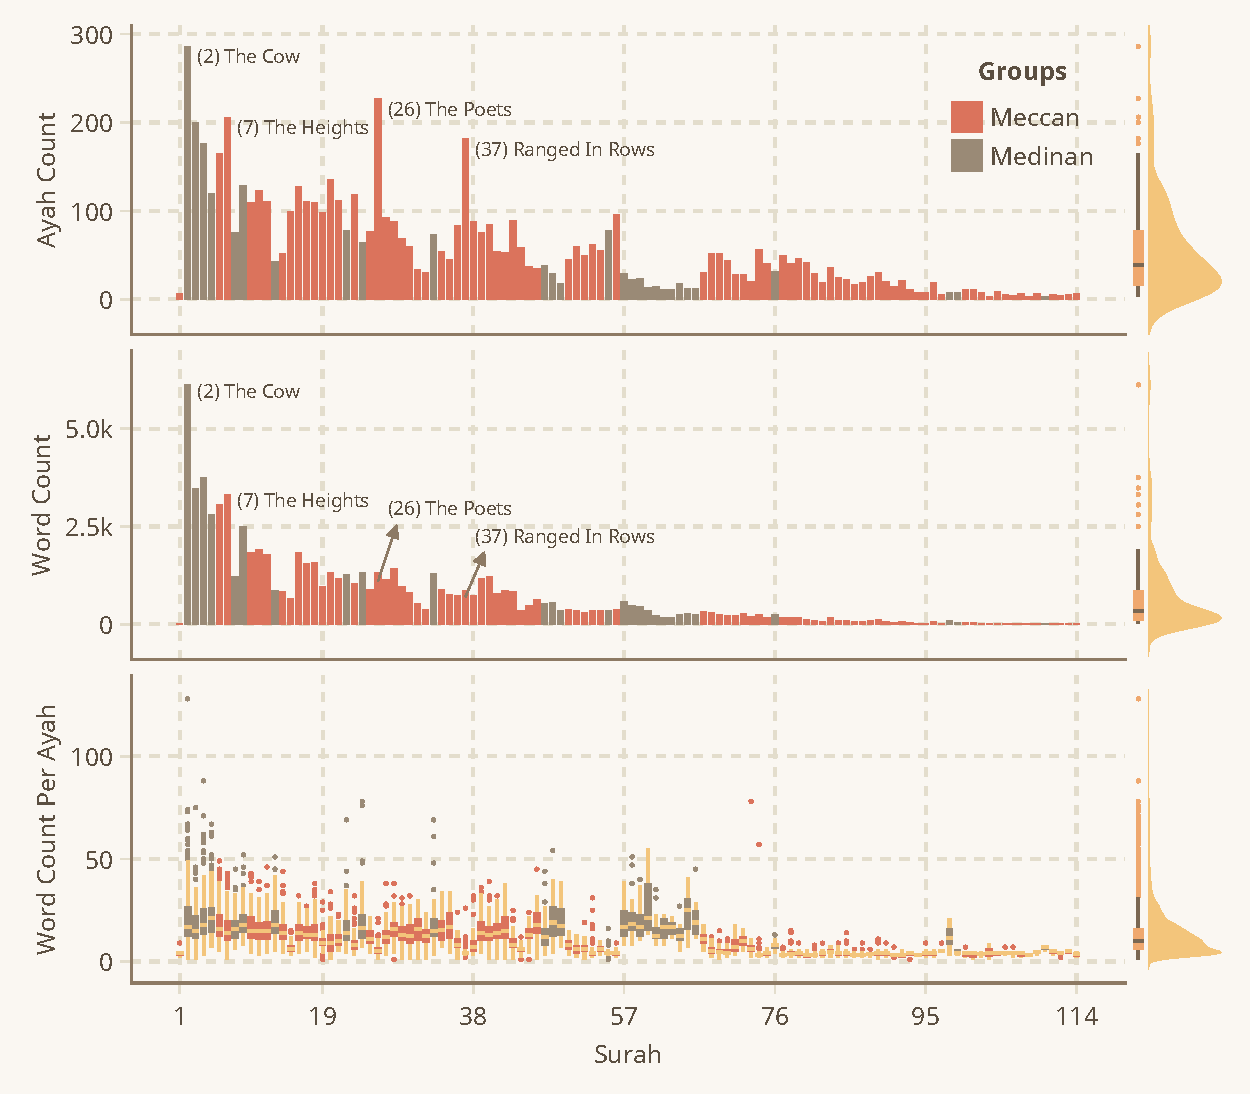
\includegraphics[width=\textwidth]{img/plot1.pdf}
    \caption{Statistics of the words and \arb[trans]{ayAt} \arb{ayAt} (verses) of the Qur'\=an}
    \label{fig:ayah_word_count_with_desc}
\end{figure}

As shown in Figure \ref{fig:ayah_word_count_with_desc}, both the Box and Density plots are tied to each other. This is indeed the case because both are describing the same information but presented in different style of visualization. In fact, Histogram is also used to describe the same information as the Box and Density, and the three are therefore related. So much so, that the three can be put into one graph. As to how to interpret these, readers are referred to for further details \textcolor{red}{[to add reference]}.
\begin{exmp}[Frequency Distribution]\label{ex:frequency_distribution}
Consider again the task of drawing an \arb[trans]{'ayAt} \arb{'ayAt} from the Qur'\=an, suppose the \arb[trans]{'ayAt} \arb{'ayAt} are separated into \arb{makkiyyaT} Meccan and \arb{madaniyyaT} Medinan, what is the probability of getting at most 10 \arb[trans]{kalimAt} \arb{kalimAt} or words in a sampled \arb[trans]{'ayAt} \arb{'ayAt} from \arb{makkiyyaT} Meccan \textit{surah}s \arb{sUr}?\\
\textit{Solution:} To answer this, Figure \ref{fig:meccan_medinan_word_count_per_ayah} shows the \textit{histograms} with the \textit{box plots} and the \textit{rainclouds} plots. The figure shows the frequency of the \arb[trans]{kalimAt} \arb{kalimAt} or words in a sampled \arb[trans]{'ayAt} \arb{'ayAt}. This frequency describes the distribution of the \arb[trans]{kalimAt} \arb{kalimAt}. To interpret this, the Medinan \arb{madaniyyaT} histogram shows that most of the \arb[trans]{'ayAt} \arb{'ayAt} have about 10 to 20 \arb[trans]{kalimAt} \arb{kalimAt} or words in total. This conclusion is based on the where the box of the box plot is located, which also corresponds to the area where the bars of the histogram are high, and also where most of the points or 'droplets' from the rainclouds plot are congested. With that said, \textit{historgram}, \textit{box plot}, and \textit{rainclouds} are related and are telling the same story from different perspectives. It should be noted that, the rainclouds plot is not a common visualization tool. 

Now, comparing the numbers from Medinan \arb{madaniyyaT} to the \arb[trans]{'AyAt 'l-makkiyyaTu} \arb{'AyAt 'l-makkiyyaTu}, there are about 5 to 15 \arb[trans]{kalimAt} \arb{kalimAt} to expect per \arb[trans]{'ayAt} \arb{'ayAt} based on Figure \ref{fig:meccan_medinan_word_count_per_ayah}. 

\begin{figure}[!t]
    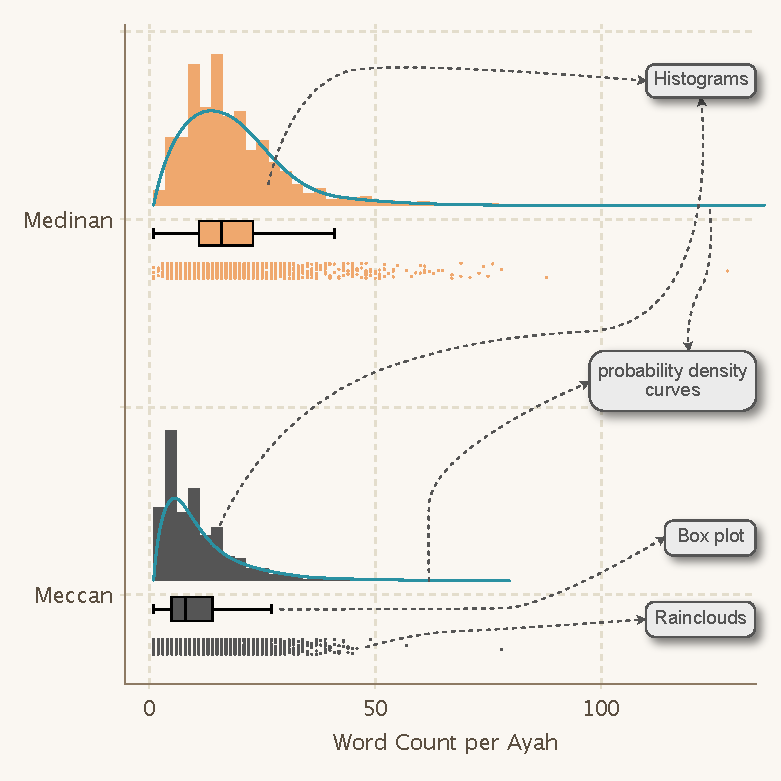
\includegraphics[width=\textwidth]{img/plot3.pdf}
    \caption{Probability density function plot of word count per \arb[trans]{'ayAt} \arb{'ayAt} by revelation location, in relation to its box plot and rainclouds.}
    \label{fig:meccan_medinan_word_count_per_ayah}
\end{figure}

The question has not been answered yet though, the above discussions only explains how to interpret the graphs in Figure \ref{fig:meccan_medinan_word_count_per_ayah}. So to answer the question, one simply needs to total the number of \arb[trans]{'AyAt} \arb{'AyAt} with at most 10 \arb[trans]{kalimAt} \arb{kalimAt} or words and divide this with the total number of \arb[trans]{'AyAt 'l-makkiyyaTu} \arb{'AyAt 'l-makkiyyaTu}. The answer is as follows, and this is part of the result of this paper: there are 4613 \arb[trans]{'AyAt 'l-makkiyyaTu} \arb{'AyAt 'l-makkiyyaTu}, and out of these is 2602 \arb[trans]{'AyAt 'l-makkiyyaTu} \arb{'AyAt 'l-makkiyyaTu} with at most 10 words. Therefore, the probability is $\frac{2602}{4613}=0.612$ or 61.2\% probability. Formally, if $X$ is the random variable of the event of observing at most 10 \arb[trans]{kalimAt} \arb{kalimAt} in a \arb[trans]{'AyAt 'l-makkiyyaTu} \arb{'AyAt 'l-makkiyyaTu}, then 
\begin{align}
     p(X\leq 10)=&\sum_{x=0}^{10} p(X=x)\label{ex_eq:prob_lesseq_10}\\
    =& p(X=0)+ p(X=1)+ p(X=2)+\cdots+ p(X=10)\label{ex_eq:freq_dist_prob1..10}\\
    =&0+\frac{24}{4613}+\frac{172}{4613}+\cdots+\frac{222}{4613}\label{ex_eq:freq_dist_probval1..10}\\
    =&\frac{2602}{4613}=0.612\label{ex_eq:prob_0612}
\end{align}

From Eq. \ref{ex_eq:freq_dist_prob1..10}, $ p(X=0)$ is the probability of observing zero \arb[trans]{kalimaT} \arb{kalimaT} in a \arb[trans]{'AyAt 'l-makkiyyaTu} \arb{'AyAt 'l-makkiyyaTu}, and $ p(X=1)$ is the probability of observing one \arb[trans]{kalimaT} \arb{kalimaT} in a \arb[trans]{'AyAt 'l-makkiyyaTu} \arb{'AyAt 'l-makkiyyaTu}, and so on. The numbers in Eq. \ref{ex_eq:freq_dist_probval1..10} are the number of \arb[trans]{'AyAt 'l-makkiyyaTu} \arb{'AyAt 'l-makkiyyaTu} having zero, one, two, to ten \arb[trans]{kalimAt} \arb{kalimAt}.

\end{exmp}
\section{Population and Sample}
Statistics is a branch of science that is concerned with understanding how the data behave based on a sample---a small set of the said data. It uses statistical methodologies to understand these behavior such as probability mass/density function, and use the findings from these tools on the sampled data as a conclusion for the population---the overall data.

Figure \ref{fig:pop_sample} illustrates the relation of population and sample data. A good example of this is the political surveys on the pulse of the nation on the candidates prior to election. Private entities like PulseAsia\footnote{\url{https://pulseasia.ph/}} and Social Weather Station\footnote{\url{https://www.sws.org.ph/swsmain/home/}} (SWS) do their survey by  sampling from the total population of the Philippines, hence the name survey.

The statistics computed from the surveys like the percentage of votes for particular political candidate are referred as estimates, this is because the computation was done in a sample of the population and not on the population itself. It is therefore important that for these estimates to be accurate representation of the nation's opinion, it has to be representative of the population. That is, the sample shouldn't be bias and leaning to the opinions of the few only and not of the whole nation.

The importance of the sample data as illustrated below follows from the fact that it saves time and cost since interviewing 2500 compared to 100,000 is better compromise for the estimated vote percentages. Further, since these samples requires to well represent the population, the computations of the statistics are estimated using statistical models, like probability mass/density functions, and other models like linear and nonlinears discussed in Section \ref{sec:stat_modeling}. The next example will illustrate the idea population and sample, and how probabilistic modeling can help in understanding insights and answering more questions.
\begin{figure}[t]
    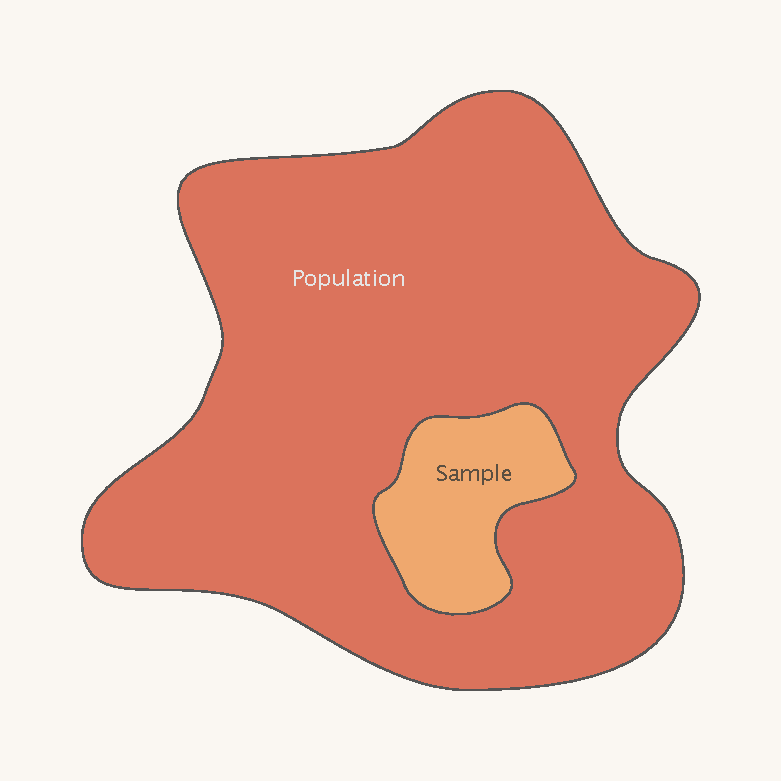
\includegraphics[width=\textwidth]{img/pop_sample.pdf}
    \caption{Population and sample illustration}
    \label{fig:pop_sample}
\end{figure}
\begin{exmp}\label{ex:population_sample_distribution_meccan_words}
Consider the task of sampling 250 \arb[trans]{'AyAt} \arb{'AyAt} from the population of \arb[trans]{'AyAt 'l-makkiyyaT}, describe the statistics of the population and the sample.\\
\textit{Solution:} In Statistics, there are several ways to sample from data, the simplest approach is through the use of \textit{uniform distribution}, that is, the sampling assumes that all data from the population are distributed equally, in the sense that all data points have equal chance of being selected. The other approach is through a \textit{weighted distribution}, where a probability is assigned to each of the data points in the population, so that, the selection will be biased to those with high probability. Figure \ref{fig:meccan_words_sampling} shows the graphs or plots of the population distribution of \arb[trans]{kalimAtu 'l-makkiyyaT} \arb{kalimAtu 'l-makkiyyaT}, which is presented as the top plot, this distribution of \arb{kalimAtu 'l-makkiyyaT} is the same one shown in the bottom plot of Figure \ref{fig:meccan_medinan_word_count_per_ayah}. 

To draw 100 samples from the said population, a simple random sampling without replacement (SRSWOR) is used for selecting or drawing samples. SRSWOR works by randomly selecting sample from the population and then setting it aside as the first sample. The resulting 100 samples are plotted in the bottom plot of Figure \ref{fig:meccan_words_sampling}.

As discussed above, the sample needs to be representative of the population. Figure \ref{fig:meccan_words_sampling} shows that the sampling distribution has more or less the same shape as the population. So that, the statistics are shown in Table \ref{tbl:meccan_words_pop_sample_stats}. From the said table, it can be seen that in terms of centrality, the both data are almost the same, for example the mean is 12.42 for the population and 10.64 for the sample. The reason why the mean in the population is much higher is due to the outlier in the population, which is seen in the extent of the tail of the Kernel Density Estimate in Figure \ref{fig:meccan_words_sampling}. In fact, this is seen in the Median in Table \ref{tbl:meccan_words_pop_sample_stats}, where  the estimate are almost the same. This is because the median is not affected by the outlier. However, the variance did suffer from the outlier in the population, with 50\% reduction in the sample variance, 54.15 to 48.96. The sample will less likely get the outlier as the sample since the outlier is only one observation from the 4163 total Meccan surahs.

The estimates got from the sample ideally are taken from a probabilistic model fitted into the sample data. This computation will be discussed in the next example.

\begin{table}
    \caption{Descriptive statistics of the population and sample data of \arb[trans]{kalimAtu 'l-makkiyyaT} \arb{kalimAtu 'l-makkiyyaT}}
    \label{tbl:meccan_words_pop_sample_stats}
    \begin{tabularx}{\textwidth}[!h]{XXXXl}
        \toprule
        Data&Mean&Median&Variance&Std. Deviation\\
        \midrule
        Population&10.28&8&54.15&7.36\\
        Sample&10.64&9&48.96&7.00\\
        \bottomrule
    \end{tabularx}
\end{table}
\begin{figure}[t]
    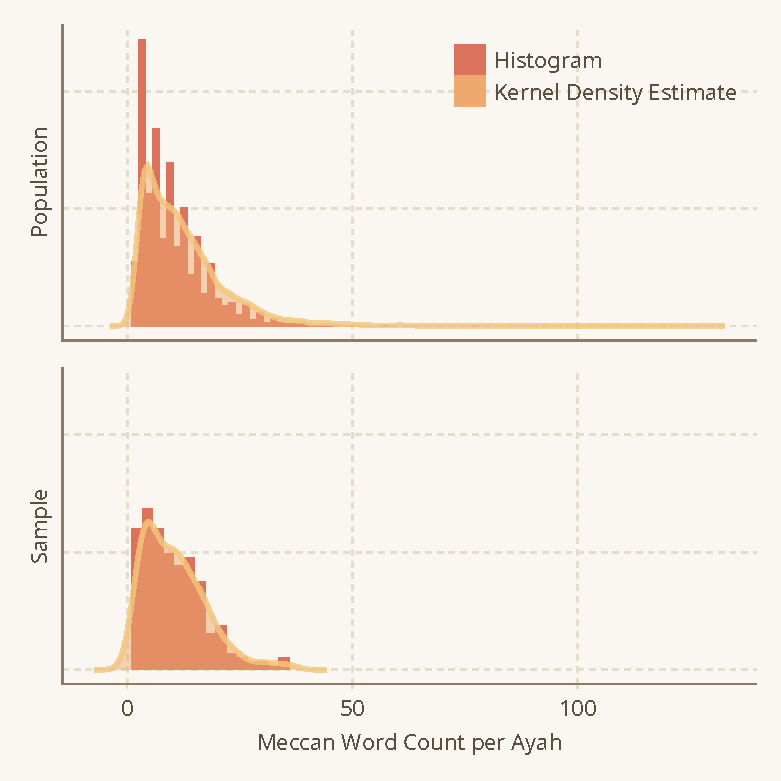
\includegraphics[width=\textwidth]{img/plot5.pdf}
    \caption{Population and sample distribution of Meccan }
    \label{fig:meccan_words_sampling}
\end{figure}

\end{exmp}
\begin{exmp}
Consider again Ex. \ref{ex:population_sample_distribution_meccan_words}, suppose the sample data is the only data available, how will you compute the probability of getting exactly 35 \arb[trans]{kalimAtu 'l-sUratu 'l-makkiyyaTu} \arb{kalimAtu 'l-sUratu 'l-makkiyyaTu}?\\
\textit{Solution:} To answer this question, one might approach this using the frequency distribution as in Ex. \ref{ex:frequency_distribution}. However, the use of frequency distribution from the said example is applicable since that deals with the population data, which is already the true probability, and there is no need to do some estimation. It is like try to get the average height of male Filipinos in the Philippines by doing census across the population, for such case, why would you do an estimate if you have all the census data of all heights of the Filipino, wouldn't it be easier to just do the average computation directly? This is the analogy for the frequency distribution used in Ex. \ref{ex:frequency_distribution}, that is, no need to do some estimation. However, for this problem, the assumption is that only the sample is available, that is, not all of the population is available. With that said, the best solution is to do some estimation. Now, doing an estimation is possible using the samples only, that is, using the idea of frequency distribution but this time applying it on the sample. This is becaus the sample was done using a random sampling, which more or less representative of the population. However, using this approach may possess a problem, let's see what that problem will likely be by forcing the approach in Ex. \ref{ex:frequency_distribution}, following the computation as in Eq. (\ref{ex_eq:prob_lesseq_10}) to Eq. (\ref{ex_eq:prob_0612}). 

Let $X$ again be the random variable of an event of observing 35 \arb[trans]{kalimAt} \arb{kalimAt}, this time from the sample, then
\begin{equation}\label{eq:probx_eq_35}
     p(X=35)=\begin{cases}
        \displaystyle\frac{0}{250}=0,&\text{if sample data}\\
        \displaystyle\frac{5}{4613}=0.0011,&\text{if population data}
    \end{cases}
\end{equation}
From the Eq. \ref{eq:probx_eq_35}, it shows that if we use the sample data for estimating the probability of observing 35 \arb{kalimAt}, then the answer above is 0, meaning by estimate there is a 0 chance of observing a 35 \arb{kalimAt} from a \arb[trans]{'AyAtu 'l-makkiyyaTu} \arb{'l-sUrAtu 'l-makkiyyaTu}. This conclusion is indeed misleading, since according to the population data, there are \arb[trans]{'AyAtu 'l-makkiyyaTu} \arb{'AyAtu 'l-makkiyyaTu} that has 35 \arb[trans]{kalimAt} \arb{kalimAt}. 

So, how to properly estimate this then? This is where the concept of probabilistic modeling comes in. For this problem, the data is count, and that the event of observing 10 \arb[trans]{kalimAtu 'l-sUratu 'l-makkiyyaTu} \arb{kalimAtu 'l-sUratu 'l-makkiyyaTu} in an \arb{'ayaT} is known to be best modeled by a Poisson distribution defined in Defn. \ref{defn:poisson_mass_function}. Ex. \ref{ex:poisson_distribution_sample} will discuss how to solve this. 
\end{exmp}
\section{Probability Distributions}
\begin{defn}[Poisson Mass Function]\label{defn:poisson_mass_function}
Let $X$ be a random variable and let $\lambda>0$ be a parameter, then if $x$ is the random value, then the \textit{Poisson} mass function is given by:
\begin{equation}
     p(X=x)=\frac{\lambda^x\exp(-\lambda)}{x!}
\end{equation}
\end{defn}
\begin{exmp}\label{ex:poisson_distribution_sample}
Consider again Ex. \ref{ex:population_sample_distribution_meccan_words}, the problem can be solved using the Poisson distribution.
\end{exmp}
\begin{defn}[Normal Density Function]
Let $Y$ be a random variable and let $\mu\in\mathbb{R}$ and $\sigma\in\mathbb{R}$ be the mean and variance parameters, if $y$ is the random value, then the \textit{Gaussian} or \textit{Normal} density function is given below:
\begin{equation}
     p(Y=y):=\frac{1}{\sqrt{2\pi\sigma^2}}\exp\left\{-\frac{(y-\mu)^2}{\sigma^2}\right\},\quad\text{where}\;-\infty<y<\infty
\end{equation}
\end{defn}
\begin{defn}[Dirichlet Density Function]
Let $\mathbf{Y}$ be a vector random variable with a random value $\mathbf{y}:=[y_1,\cdots,y_k]^{\text{T}}$ and let $\boldsymbol{\alpha}:=[\alpha_1,\cdots,\alpha_k]^{\text{T}}$ be the parameters, then the \textit{Dirichlet} density function is defined as
\begin{equation}
     p(\mathbf{X}=\mathbf{x};\boldsymbol{\alpha}):=\frac{1}{B(\boldsymbol{\alpha})}\prod_{i=1}^kx_i^{\alpha_i-1},
\end{equation}
where,
\begin{equation}
    B(\boldsymbol{\alpha}):=\frac{\displaystyle\prod_{i=1}^k\Gamma(\alpha_i)}{\Gamma\left(\sum_{i=1}^k\alpha_i\right)}
\end{equation}

\end{defn}
\begin{defn}[Multinomial Mass Function]
Let $\mathbf{X}$ be a vector random variable with a random value $\mathbf{x}:=[x_1,\cdots,x_k]^{\text{T}}$ such that $x_i\geq 0,\forall i \in[1,k]$, let $\boldsymbol{q}:=[q_1,\cdots,q_k]^{\text{T}}$ and $n$ be the parameters, the probability mass function of a Multinomial distribution is 
\begin{align}
    f(x_1,\cdots,x_k;n,q_1,\cdots,q_k):=& q(X_1=x_1\;\text{and}\;\cdots\;\text{and}\;X_k=x_k)\nonumber\\
    =&\begin{cases}
        \displaystyle\frac{n!}{x_1!\cdots x_k!}q_1^{x_1}\times\cdots\times q_k^{x_k},&\text{when}\;\sum_{i=1}^kx_i=n\\
        0&\text{otherwise},
    \end{cases}
\end{align}
\end{defn}

\section{Frequentist Estimation}\label{sec:stat_modeling}
Probability distributions are fundamental models that can be used to describe some characteristics of the data. However, combinations of variables, and accounting dynamics of the observations can lead into other types of models as well. In general, a statistical model can be written using the following formula:
\begin{equation}
    y=f(x|\mathbf{\Theta})+\varepsilon,
\end{equation}
where $y\sim p(\cdot)$ and $\varepsilon\sim p(\cdot)$.

There are two main ways to estimating the parameters $\boldsymbol{\Theta}$, and that is either through Frequentist or Bayesian approach.
\subsection{Maximum Likelihood Estimation}
Maximum likelihood estimation (MLE) is a fundamental concept in statistics that provides a method for estimating the parameters of a statistical model based on the observed data. The basic idea behind MLE is to find the parameter values that make the observed data most likely or probable under the assumed statistical model. The concept of MLE can be explained as follows:

Suppose we have a random sample of observations $X := \{x_1, x_2, ..., x_n\}$ from a probability distribution $f(x | \theta)$, where $\theta$ represents the unknown parameter(s) of the distribution. The likelihood function, denoted as $\mathcal{L}(\theta | X)$, is the joint probability density (or probability mass function for discrete distributions) of the observed data $X$, treated as a function of the parameter(s) $\theta$.
\begin{equation}
    \mathcal{L}(\theta | X) = f(x_1 | \theta) \times f(x_2 | \theta) \times\cdots\times f(x_n | \theta)    
\end{equation}

The maximum likelihood estimate (MLE) of $\theta$, denoted as $\hat{\theta}$, is the value of $\theta$ that maximizes the likelihood function $\mathcal{L}(\theta | X)$. In other words, $\hat{\theta}$ is the value of θ that makes the observed data most likely or probable under the assumed statistical model.
\begin{equation}
    \hat{\theta} = \underset{\theta}{\arg\max} \mathcal{L}(\theta | X)    
\end{equation}

In practice, it is often easier to work with the log-likelihood function, denoted as $\ell(\theta | X) = \log(\mathcal{L}(\theta | X))$, since the logarithm is a monotonic function and maximizing the log-likelihood is equivalent to maximizing the likelihood.
\begin{equation}
   \hat{\theta} = \underset{\theta}{\arg\max}\ell(\theta | X)    
\end{equation}
\begin{exmp}[Normal distribution]
    Suppose we have a random sample $X = \{x_1, x_2,\cdots, x_n\}$ from a normal distribution with unknown mean μ and known variance $\sigma^2$. The likelihood function is:
    \begin{equation}
        \mathcal{L}(\mu | X) = \frac{1}{(\sqrt{2\pi\sigma^2})^n}\exp\left(-\sum_{\forall i}(x_i - \mu)^2 / (2\sigma^2)\right)
    \end{equation}
    
    Taking the log and differentiating with respect to $\mu$, setting the derivative equal to zero, and solving for $\mu$, we get the maximum likelihood estimate or MLE of $\mu$:
    \begin{equation}
        \hat{\mu} = \frac{1}{n}\sum_{\forall i}x_i
    \end{equation}
\end{exmp}
MLE has several desirable properties, such as consistency (the MLE converges to the true parameter value as the sample size increases) and asymptotic normality (the sampling distribution of the MLE approaches a normal distribution as the sample size increases), which make it a widely used method in statistical inference and modeling.
\subsection{Numerical Approximation}
There are several ways to numerically estimate the parameters of the model using mathematical programming. The popular algorithm that is very common in Machine Learning is the \textit{gradient descent} (GD) given in Algorithm \ref{algo:GD}. Suppose $\nabla\ein(\hat{\mathbf{w}}^{(r)})$ is the gradient of the cost function at the $r$th iteration. $\ein$ is defined as \mbox{the \textit{in-sample error}} or the error in the training dataset, $\gamma$ is the \textit{learning-rate} parameter of the algorithm and $\nu$ is the \textit{precision} parameter. As an illustration, consider Example \ref{ex:gd}.\vspace{.4cm}

\begin{algorithm}
\caption{\it Gradient Descent}
\label{algo:GD}
\begin{algorithmic}[1]\vspace{.2cm}
\item Initialize $\hat{\mathbf{w}}^{(r)},r=0$\vspace{.2cm}
\While{$\lVert \hat{\mathbf{w}}^{(r+1)}-\hat{\mathbf{w}}^{(r)}\rVert > \nu$}\vspace{.2cm}
\State $\hat{\mathbf{w}}^{(r+1)}\triangleq \hat{\mathbf{w}}^{(r)} - \gamma\nabla\ein(\hat{\mathbf{w}}^{(r)})$\vspace{.2cm}
\State $r\triangleq r + 1$\vspace{.2cm}
\EndWhile\\\vspace{.2cm}
\Return $\hat{\mathbf{w}}^{(r)}$ and $r$.
\end{algorithmic}
\end{algorithm}
\vspace{-.3cm}

\begin{exmp}\label{ex:gd}
Suppose the loss function is given by
\begin{equation}\label{eq:errgd1}
\ein(w)\triangleq w^4 - 3w^3 + 2.
\end{equation}
The first derivative of the above equation with respect to $w$ is given by ${\ein'(w)=4w^3-9w^2}$. Let the initial guess be $\hat{w}^{(0)}=.1$ and let $\gamma=.01$ with $\nu=.00001$. Then $\nabla\ein(\hat{w}^{(0)})=\ein'(\hat{w}^{(0)})=-0.086$, so that $\hat{w}^{(1)}\triangleq\hat{w}^{(0)}-.01(-0.086)=0.10086$, and $|\hat{w}^{(1)} - \hat{w}^{(0)}| = 0.00086> \nu$. It turns out that 173 iterations are needed to satisfy \mbox{the inequality}, $|\hat{w}^{(r+1)} - \hat{w}^{(r)}| \ngtr \nu$.
\end{exmp}
In practice, however, there are hundreds to millions of data points that need to be summarized, so that at each iteration, the parameters are updated \textit{after} \mbox{the presentation} of \textit{all} the training examples that constitute an \textit{epoch} --- one complete presentation of the entire training dataset during the learning process \cite{Haykin1998}. In this setting, GD is sometimes called \textit{batch gradient descent} (BGD).
\subsection{Stochastic Gradient Descent}\label{sec:sgd}
An alternative to BGD is SGD or \textit{stochastic gradient descent}. SGD updates the parameter using only one observation for every iteration, which is a lot faster. Further, BGD is prone to local minimum since GD does so. This is guaranteed for misspecified initial value especially for high dimensional nonlinear error surface function. \mbox{The stochasticity} of the SGD follows from the randomization of the dataset at each epoch, and contrary to BGD, the SGD is not expected to converge to \mbox{the global} minimum, instead it will only stay around the global solution (\textit{see} Algorithm \ref{algo:SGD}). Example \ref{exmp:bgdslr} illustrates the application of mathematical programming in estimating the parameters of a simple linear regression model.
\vspace{.4cm}

\begin{algorithm}[!h]
\caption{\it Stochastic Gradient Descent}
\label{algo:SGD}
\begin{algorithmic}[1]\vspace{.2cm}
\item Initialize $\hat{\mathbf{w}}^{(r)},r=0$\vspace{.2cm}
\While{$\lVert \hat{\mathbf{w}}^{(r)}-\hat{\mathbf{w}}^{(r+1)}\rVert > \nu$}\vspace{.2cm}
\State Randomize the data set ($\mathbf{x}_i,\mathbf{y}_i$) with respect to $i$.\vspace{.2cm}
\For{$i \in\{1,\cdots, n\}$}\vspace{.2cm}
\State Update the parameters
\begin{align}\nonumber
\hat{\mathbf{w}}^{(r)}&\triangleq \hat{\mathbf{w}}^{(r)} - \gamma\nabla\mathrm{e}(h(\mathbf{x}_i,\hat{\mathbf{w}}^{(r)}),\mathbf{y}_i)\\\nonumber
&=\hat{\mathbf{w}}^{(r)} - \gamma\frac{\partial}{\partial\mathbf{w}}\left\{\frac{1}{2}[h(\mathbf{x}_i,\hat{\mathbf{w}}^{(r)})-\mathbf{y}_i]^2\right\}
\end{align}
%\State Compute $\mathrm{e}^{(r)}\triangleq\mathrm{e}(h(\mathbf{x}_k,\hat{\mathbf{w}}^{(r+1)}),\mathbf{y}_k)$\vspace{.2cm}
\EndFor\vspace{.2cm}
\State $\hat{\mathbf{w}}^{(r+1)}\triangleq \hat{\mathbf{w}}^{(r)}$\vspace{.2cm}
%\State Compute the cost function
%\begin{equation}
%\ein(h)=\frac{1}{n}\sum_{i=1}^K\mathrm{e}(h(\mathbf{x}_i,\hat{\mathbf{w}}^{(r+1)}),\mathbf{y}_i)
%\end{equation}
\EndWhile\vspace{.2cm}
\item\Return $\hat{\mathbf{w}}^{r}$ and $r$.
\end{algorithmic}
\end{algorithm}
\section{Bayesian Estimation}
Bayesian estimation is a statistical approach that incorporates prior knowledge or beliefs about the parameters of interest into the estimation process. It combines the prior knowledge with the observed data to obtain updated beliefs or estimates of the parameters, known as the posterior distribution.
The Bayesian estimation framework is based on Bayes' theorem, which relates the conditional probabilities of events. In the context of parameter estimation, Bayes' theorem can be expressed as:
\begin{equation}
    p(\theta | X) = \frac{p(X | \theta)p(\theta))}{p(X)}
\end{equation}
where $p(\theta | X)$ is the posterior distribution, representing the updated beliefs about the parameter(s) $\theta$ after observing the data X. $p(X | \theta)$ is the likelihood function, which quantifies the probability of observing the data X given the parameter(s) $\theta$. $p(\theta)$ is the prior distribution, representing the initial beliefs or knowledge about the parameter(s) $\theta$ before observing the data. $p(X)$ is the marginal likelihood or the probability of observing the data X, which acts as a normalizing constant.
\subsection{Laplace's Approximation}\label{sec:laplace}
The simplest approximation to the posterior distribution of the parameter of interest is the Laplace's approximation. The idea behind this procedure is to use a Gaussian approximator, $\g(x)$, such that it is centered on the mode of the target distribution, $ p(x)$. To illustrate, suppose
\begin{equation}
 p(x):=\frac{f(x)}{Z},\quad\mathrm{where}\;Z:=\int f(x)\D x.
\end{equation}
Using basic calculus, the mode\footnote{obtained using maximum \textit{a posteriori} (MAP)} of the posterior distribution, say at $x=x_{\text{MAP}}$, is achieved by taking the derivative of the objective function with respect to the $x$-axis, such that the gradient of the function is $0$ at $x=x_{\text{MAP}}$. That is,
\begin{equation}
\frac{\D f(x)}{\D x}\bigg|_{x=x_{\text{MAP}}}=0.
\end{equation}
The Gaussian distribution has the property that its logarithm is a quadratic function of the variables \cite{bishop}. Hence, the following is an approximation of \mbox{the log} of \mbox{the objective} function using second-order Taylor series expansion centered on \mbox{the mode} $x_{\text{MAP}}$, 
\begin{align}
\log f(x)=&\log f(x_{\text{MAP}})+\frac{\D \log f(x)}{\D x}\bigg|_{x=x_{\text{MAP}}}(x-x_{\text{MAP}})\\
&+\frac{\D^2 \log f(x)}{\D x^2}\bigg|_{x=x_{\text{MAP}}}\frac{(x-x_{\text{MAP}})^2}{2}+\mathcal{O}(x)\\
\approx&\log f(x_{\text{MAP}})+\frac{\D^2 \log f(x)}{\D x^2}\bigg|_{x=x_{\text{MAP}}}\frac{(x-x_{\text{MAP}})^2}{2}.
\end{align}
Exponentiating both sides of the above equations becomes
\begin{equation}
f(x)\approx f(x_{\text{MAP}})\exp\left[\frac{\D^2 \log f(x)}{\D x^2}\bigg|_{x=x_{\text{MAP}}}\frac{(x-x_{\text{MAP}})^2}{2}\right],
\end{equation}
so that the normalized estimator $\g(x)$ is given by
\begin{equation}
\g(x)=\left(-\frac{1}{2\pi}\frac{\D^2 \log f(x)}{\D x^2}\bigg|_{x=x_{\text{MAP}}}\right)^{1/2}\exp\left[\frac{\D^2 \log f(x)}{\D x^2}\bigg|_{x=x_{\text{MAP}}}\frac{(x-x_{\text{MAP}})^2}{2}\right].
\end{equation}
\vspace{-1cm}
\begin{exmp}
Suppose the posterior distribution is a chi-square of the form: $p(x):=\frac{x^{k-1}\exp\left(-\frac{x^2}{2}\right)}{Z}$, with $k$ degrees of freedom where $Z:=2^{\frac{k}{2}-1}\Gamma\left(\frac{k}{2}\right),\quad x>0$. Using Laplace, \mbox{the approximator} to the posterior distribution is obtained as follows:\\[.3cm]
The log-likelihood of the density function is given by
\begin{equation}
\ell(x):=\log p(x)=(k-1)\log x-\frac{x^2}{2}+\mathcal{C},
\end{equation}
where $\mathcal{C}$ is the constant. The mode of this posterior is given by
\begin{align}
\frac{\partial}{\partial x}\log  p(x)&=\frac{k-1}{x_{\text{MAP}}}-x_{\text{MAP}}\overset{\text{set}}{=}0\\
x_{\text{MAP}}&=\sqrt{k-1}.
\end{align}
The second partial derivative of the log-likelihood with respect to $x$ evaluated at $x_{\text{MAP}}$ is
\begin{equation}\label{eq:laplaceexapprox}
-\frac{\partial^2}{\partial x^2}\log  p(x)\bigg|_{x=x_{\text{MAP}}}=1-\frac{1-k}{x_{\text{MAP}}^2}=2.
\end{equation}
Thus the estimate of the posterior is given by a Gaussian distribution with mean $\mu=\sqrt{k-1}$ and variance $\sigma^2 = \frac{1}{2}$. Figure \ref{fig:laplaceapprox} visualizes the Gaussian distribution as an approximator to the posterior distribution.
\end{exmp}
Now consider the case where $\mathbf{x}\in\mathbb{R}^{d}$, such that $ p(\mathbf{x}):=\frac{f(\mathbf{x})}{Z}$. Analogous to \mbox{the univariate} case, the Laplace's approximation for $ p(\mathbf{x})$ is obtained by aligning \mbox{the mean} of the multivariate Gaussian distribution to the mode of the posterior density, denoted by $\mathbf{x}_{\text{MAP}}$. As before, the log-likelihood of $f(\mathbf{z})$ is given by \mbox{the following} equation
\begin{equation}\label{eq:laplacemultivar}
\log f(\mathbf{x})\approx\log f(\mathbf{x}_{\text{MAP}})-\frac{1}{2}(\mathbf{x}-\mathbf{x}_{\text{MAP}})^{\text{T}}\boldsymbol{\mathfrak{H}}(\mathbf{x}-\mathbf{x}_{\text{MAP}}),
\end{equation}
where $\boldsymbol{\mathfrak{H}}$ is the Hessian matrix defined by
\begin{equation}\label{eq:2ndderivlaplace}
\boldsymbol{\mathfrak{H}}:=-\frac{\partial^2}{\partial\mathbf{x}^2}\log f(\mathbf{x})\bigg|_{\mathbf{x}=\mathbf{x}_{\text{MAP}}}.
\end{equation}
Exponentiating Equation (\ref{eq:laplacemultivar}) leads to the normalized approximator, $\g(\mathbf{x})=\mathcal{N}_d(\mathbf{x}|\mathbf{x}_{\text{MAP}},\boldsymbol{\mathfrak{H}}^{-1})$.
\subsection{Markov Chain Monte Carlo (MCMC)}
Laplace has the advantage of being simple and easy to use. However, like any approximator, it has limitations especially on multimodal densities since it uses Gaussian as estimate to the posterior distribution. Most interesting high dimensional Bayesian models have multimodal \textit{a posteriori}, which can't be captured through Laplace's method. To address this problem, sampling methods are instead used for approximating the \textit{a posteriori}. These family of sampling methods are called Markov Chain Monte Carlos (MCMC) with \textit{Metropolis-Hasting} (MH) and \textit{Gibbs sampling} as \mbox{the popular} MCMCs. Further, for sophisticated MCMCs, the algorithms available are not limited to \textit{Hamiltonian Monte Carlo} (HMC) and \textit{Stochastic Gradient HMC}.
\subsection{Metropolis-Hasting}\label{sec:metropolishasting}
The idea of the MH algorithm is to randomly walk in the support of the target density such that the random step is governed by the proposal distribution $\g(\cdot)$. \mbox{The assumption} is that the posterior distribution has no closed-form solution, but the kernel, which is the unnormalized form of the target density is easy to evaluate. This is the advantage of the Metropolis-Hasting algorithm where the \textit{a posteriori} is not necessarily be normalized --- often the difficulty in simplifying the model evidence of the Bayes' rule. Let $ p(\cdot)$ be the \textit{a posteriori}, then the Metropolis-Hasting algorithm is given in Algorithm \ref{algo:mcmcmh}.
\vspace{.4cm}

\begin{algorithm}[!t]
\caption{\it Metropolis-Hasting MCMC}
\label{algo:mcmcmh}
\begin{algorithmic}[1]\vspace{.2cm}
\item Initialize $\mathbf{w}_{r}\sim\g(\mathbf{w}),r=0$\vspace{.2cm}
\For {$r\in\{1,\cdots, r_{\text{max}}\}$}\vspace{.2cm}
\State Propose: $\mathbf{w}_{new}\sim\g(\mathbf{w}_{new}|\mathbf{w}_{r-1})$\vspace{.2cm}
\State Acceptance: $\alpha(\mathbf{w}_{new}|\mathbf{w}_{r-1}):=\min\left\{1,\frac{ p(\mathbf{w}_{new}|\mathbf{w}_{r-1})\g(\mathbf{w}_{r-1}|\mathbf{w}_{new})}{ p(\mathbf{w}_{r-1}|\mathbf{w}_{new})\g(\mathbf{w}_{new}|\mathbf{w}_{r-1})}\right\}$\vspace{.2cm}
\State Draw $x\sim\text{Unif}(0,1)$\vspace{.2cm}
\If {$x<\alpha(\mathbf{w}_{new}|\mathbf{w}_{r-1})$}\vspace{.2cm}
\State $\mathbf{w}_{r}:=\mathbf{w}_{new}$
\vspace{.2cm}
\Else \vspace{.2cm}
\State $\mathbf{w}_{r}:=\mathbf{w}_{r-1}$\vspace{.2cm}
\EndIf\vspace{.2cm}
\EndFor
\end{algorithmic}
\end{algorithm}
\vspace{-.3cm}
\begin{exmp}\label{exmp:mcmcmh}
Consider the bivariate Gaussian distribution defined below:
\begin{equation}
f(\mathbf{x}|\boldsymbol{\mu},\boldsymbol{\Sigma})
:=\frac{1}{\sqrt{(2\pi)^d|\boldsymbol{\Sigma}|}}\exp\left[-\frac{1}{2}(\mathbf{x} - \boldsymbol{\mu})^{\text{T}}\boldsymbol{\Sigma}^{-1}(\mathbf{x}-\boldsymbol{\mu})\right].
\end{equation}
Suppose it has the following parameters: 
\begin{equation}\nonumber
\boldsymbol{\mu}:=[10\;-10]^{\text{T}} \quad\text{and}\quad \boldsymbol{\Sigma}:=\left[\begin{array}{cc}1.5^2&\rho(1.5)(1.35)\\\rho(1.5)(1.35)&1.35^2\end{array}\right]
\end{equation}
where ${\rho := .5}$; in order to draw samples from this model, let the proposal distribution defined to be the current step of the random walk plus an increment from a uniform distribution with parameters min = -5 and max = 5.

The random samples drawn by MH are not independent, this is due to \mbox{the design} of the algorithm where the distribution of the candidate sample depends solely on the current sample\footnote{this is the property of the Markov Chain, hence the name MCMC.}. To address this problem, diagnostics are applied using methods such as \textit{thinning}, where every $i$th sample is taken and the rest are discarded; or using \textit{burn-in} where first $n^{\star}$ samples are discarded.

\end{exmp}
\subsection{Gibbs Sampling}\label{sec:gibbssampling}
MH is by far one of the easiest MCMC algorithm for drawing samples from \textit{a posteriori} where direct sampling is not possible. It uses proposal distribution as drivers of the random walk in the support of the target density, which for high dimensional data, the choice of appropriate proposal function is sometimes difficult to specify. As an alternative, Gibbs sampler can be used for taking samples from the posterior distribution. The only requirement is that the joint distribution of the parameters (the \textit{a posteriori}) can be decomposed into conditional distributions of each variable conditioned on other variables. Mathematically, suppose \mbox{the multivariate} distribution is given by $f(\mathbf{w}|\mathscr{D})$, where $\mathbf{w}:=[w_1\;w_2\cdots w_K]^{\text{T}}$, then the Gibbs sampling algorithm is given in Algorithm \ref{algo:mcmcgibbs}.
\vspace{.4cm}

\begin{algorithm}[!b]
\caption{\it Gibbs Sampling MCMC}
\label{algo:mcmcgibbs}
\begin{algorithmic}[1]\vspace{.2cm}
\item Initialize $\mathbf{w}_{r}, r=0$\vspace{.2cm}
\For {$r\in\{1,\cdots, r_{\text{max}}\}$}\vspace{.2cm}
\State $w_1^{(new)}\sim f(w_1|w_2,\cdots,w_K)$\vspace{.2cm}
\State $w_2^{(new)}\sim f(w_2|w_1^{(new)},\cdots,w_K)$\vspace{.2cm}
\State $w_3^{(new)}\sim f(w_3|w_1^{(new)},w_2^{(new)},\cdots,w_K)$\vspace{.2cm}
\State $\vdots\qquad\qquad\qquad\vdots\qquad\qquad\qquad\vdots$\vspace{.2cm}
\State $w_K^{(new)}\sim f(w_K|w_1^{(new)},w_2^{(new)},\cdots,w_{K-1}^{(new)})$\vspace{.2cm}
\State $\mathbf{w}_r:=[w_1^{(new)},\cdots,w_K^{(new)}]^{\text{T}}$\vspace{.2cm}
\EndFor
\end{algorithmic}
\end{algorithm}
\vspace{-.3cm}
\begin{exmp}\label{exmp:gibbs}
Using the same posterior distribution as in Example \ref{exmp:mcmcmh}, the conditional distributions of the parameters conditioned on other parameters are also Gaussian with mean $\mu:=\mu_1 + \left(\frac{\sigma_1}{\sigma_2}\right)\rho(x - \mu_2)$ and standard deviation $\sigma:=\sqrt{(1 - \rho^2)\sigma_1^2}$. Analogous to MH, samples obtained using Gibbs are not independent but with lower autocorrelation compared to the former. As before, the same diagnostics can be done. 
\end{exmp}
\subsection{Bayesian Linear Regression}\label{sec:blr}
As an illustration of Bayesian inference to basic modeling, this section attempts to discuss the Bayesian approach to linear regression. Let ${\mathscr{D}=\{(\mathbf{x}_1,y_1),\cdots, (\mathbf{x}_n,y_n)\}}$ where $\mathbf{x}_i\in\mathbb{R}^{d}, y_i\in \mathbb{R}$ be the pairwised dataset. Suppose the response values, $y_1,\cdots,y_n$, are independent given the parameter $\mathbf{w}$, and is distributed as $y_i\sim\mathcal{N}(\mathbf{w}^{\text{T}}\mathbf{x}_i,\alpha^{-1})$, where $\alpha^{-1}$ is referred to as the \textit{precision} parameter --- useful for later derivation. In Bayesian perspective, the weights are assumed to be random and are governed by some \textit{a priori} distribution. The choice of this distribution is subjective, but choosing arbitrary \textit{a priori} can sometimes or often result to an intractable integration, especially for interesting models. For simplicity, a conjugate prior is used for the latent weights. Specifically, assume that ${\mathbf{w}\sim\mathcal{N}(\mathbf{0},\beta^{-1}\mathbf{I})}$ such that $\beta>0$ is the hyperparameter supposed in this experiment as known value. The posterior distribution based on the Bayes' rule is given by
\begin{equation}\label{eq:bayesrulepost}
	p(\mathbf{w}|\mathbf{y})=\frac{p(\mathbf{w})p(\mathbf{y}|\mathbf{w})}{p(\mathbf{y})},
\end{equation}
where $p(\mathbf{w})$ is the \textit{a priori} distribution of the parameter, $p(\mathbf{y}|\mathbf{w})$ is the likelihood, and $p(\mathbf{y})$ is the normalizing factor. The likelihood is given by
\begin{align}
    p(\mathbf{y}|\mathbf{w})&=\prod_{i=1}^{n}\frac{1}{\sqrt{2\pi\alpha^{-1}}}\exp\left[-\frac{\alpha(y_i-\mathbf{w}^{\text{T}}\mathbf{x}_i)^2}{2}\right]\\
    &=\left(\frac{\alpha}{2\pi}\right)^{n/2}\exp\left[-\sum_{i=1}^n\frac{\alpha(y_i-\mathbf{w}^{\text{T}}\mathbf{x}_i)^2}{2}\right].\label{eq:likelihood:blreg}
\end{align}
In matrix form, this can be written as
\begin{equation}
    p(\mathbf{y}|\mathbf{w})\propto\exp\left[-\frac{\alpha}{2}(\mathbf{y}-\boldsymbol{\mathfrak{A}}\mathbf{w})^{\text{T}}(\mathbf{y}-\boldsymbol{\mathfrak{A}}\mathbf{w})\right]
\end{equation}
where $\boldsymbol{\mathfrak{A}}=\left[(\mathbf{x}_i^{\text{T}})\right]$, i.e. $\boldsymbol{\mathfrak{A}}\in(\mathbb{R}^{n}\times\mathbb{R}^d)$, this matrix is known as the \textit{design matrix}. Given that $\mathbf{w}$ has the following prior distribution
\begin{equation}\label{eq:wpriori}
    p(\mathbf{w})=\frac{1}{\sqrt{(2\pi)^{d}|\beta^{-1}\mathbf{I}|}}\exp\left[-\frac{1}{2}\mathbf{w}^{\text{T}}\beta\mathbf{I}\mathbf{w}\right],
\end{equation}
implies that the posterior has the following form:
\begin{align}
    p(\mathbf{w}|\mathbf{y})&\propto\exp\left[-\frac{\alpha}{2}(\mathbf{y}-\boldsymbol{\mathfrak{A}}\mathbf{w})^{\text{T}}(\mathbf{y}-\boldsymbol{\mathfrak{A}}\mathbf{w})\right]\exp\left[-\frac{1}{2}\mathbf{w}^{\text{T}}\beta\mathbf{I}\mathbf{w}\right]\\
&=\exp\left\{-\frac{1}{2}\left[\alpha(\mathbf{y}-\boldsymbol{\mathfrak{A}}\mathbf{w})^{\text{T}}(\mathbf{y}-\boldsymbol{\mathfrak{A}}\mathbf{w})+\mathbf{w}^{\text{T}}\beta\mathbf{I}\mathbf{w}\right]\right\}.
\end{align}
Expanding the terms in the exponent, becomes
\begin{equation}\label{eq:expterms}
    \alpha\mathbf{y}^{\text{T}}\mathbf{y}-2\alpha\mathbf{w}^{\text{T}}\boldsymbol{\mathfrak{A}}^{\text{T}}\mathbf{y}+\mathbf{w}^{\text{T}}(\alpha\boldsymbol{\mathfrak{A}}^{\text{T}}\boldsymbol{\mathfrak{A}}+\beta\mathbf{I})\mathbf{w}.
\end{equation}
The next step is to complete the square of the above equation such that it resembles the inner terms of the exponential factor of the Gaussian distribution. The quadratic form of the exponential term of a $\mathcal{N}(\mathbf{w}|\boldsymbol{\mu},\boldsymbol{\Sigma}^{-1})$ is given by
\begin{align}
    (\mathbf{w}-\boldsymbol{\mu})^{\text{T}}\boldsymbol{\Sigma}^{-1}(\mathbf{w}-\boldsymbol{\mu})&=(\mathbf{w}-\boldsymbol{\mu})^{\text{T}}(\boldsymbol{\Sigma}^{-1}\mathbf{w}-\boldsymbol{\Sigma}^{-1}\boldsymbol{\mu})\\
&=\mathbf{w}^{\text{T}}\boldsymbol{\Sigma}^{-1}\mathbf{w}-
2\mathbf{w}^{\text{T}}\boldsymbol{\Sigma}^{-1}\boldsymbol{\mu}+\boldsymbol{\mu}^{\text{T}}\boldsymbol{\Sigma}^{-1}\boldsymbol{\mu}.\label{eq:expnorm}
\end{align}
The terms in Equation (\ref{eq:expterms}) are matched up with that in (\ref{eq:expnorm}), so that
\begin{equation}\label{eq:sigmablrgauss}
    \boldsymbol{\Sigma}^{-1}=\alpha\boldsymbol{\mathfrak{A}}^{\text{T}}\boldsymbol{\mathfrak{A}}+\beta\mathbf{I}
\end{equation}
and
\begin{align}
    \mathbf{w}^{\text{T}}\boldsymbol{\Sigma}^{-1}\boldsymbol{\mu}&=\alpha\mathbf{w}^{\text{T}}\boldsymbol{\mathfrak{A}}^{\text{T}}\mathbf{y}\\
    \boldsymbol{\Sigma}^{-1}\boldsymbol{\mu}&=\alpha\boldsymbol{\mathfrak{A}}^{\text{T}}\mathbf{y}\\
    \boldsymbol{\mu}&=\alpha\boldsymbol{\Sigma}\boldsymbol{\mathfrak{A}}^{\text{T}}\mathbf{y}.\label{eq:mublrgauss}
\end{align}
Thus the \textit{a posteriori} is a Gaussian distribution with location parameter in \mbox{Equation (\ref{eq:mublrgauss})} and scale parameter given by the inverse of Equation (\ref{eq:sigmablrgauss}).
\section{Types of Statistical Methods}
\textit{Parametric} and \textit{non-parametric} statistics are two broad categories of statistical methods, each with its own assumptions and applications. The primary difference between them lies in the underlying assumptions made about the population distribution.
\subsection{Parametric}
Parametric statistics are based on the assumption that the data follows a specific probability distribution, such as the normal distribution (also known as the Gaussian distribution). These methods rely on the estimation of parameters (such as the mean and standard deviation) from the sample data to make inferences about the population.
\begin{enumerate}
    \item \textbf{Student's t-test} - for comparing means
    \item \textbf{Analysis of Variance (ANOVA)} - for comparing means across multiple groups
    \item \textbf{Pearson's correlation coefficient} - for measuring linear correlation
    \item \textbf{Linear regression} - for modeling relationships between variables
\end{enumerate}
\subsection{Nonparametric}
Non-parametric statistics, also known as distribution-free tests, do not make assumptions about the underlying probability distribution of the data. These methods are based on the ranks or signs of the data rather than the actual values.
\begin{enumerate}
    \item \textbf{Mann-Whitney U test} - for comparing two independent groups
    \item \textbf{Wilcoxon signed-rank test} - for comparing two related groups or paired samples
    \item \textbf{Kruskal-Wallis test} - for comparing more than two independent groups
    \item \textbf{Spearman's rank correlation coefficient} - for measuring monotonic relationships between variables
\end{enumerate}
\section{Types of Models}
Generally, there are two types of models, the \textit{supervised} and \textit{unsupervised}. The other one that is not common, is the \textit{semi-supervised}. The following sections will elaborate more.
\subsection{Supervised}
Supervised learning models are trained using labeled data, which means that each training example is paired with an output label. The goal is to learn a mapping from inputs to outputs based on the labeled training data, so the model can predict the output for new, unseen inputs. The following are examples of supervised learning models:
\begin{enumerate}
    \item \textbf{Linear Regression} - used for predicting continuous outcomes that are not time dependent.
    \item \textbf{Logistic Regression} - used for binary classification.
    \item \textbf{Neural Networks} - the core model powering most of the big AI models and applications.
\end{enumerate}
\subsection{Unsupervised}\label{sec:unsupervised_models}
Unsupervised learning models are trained using unlabeled data, which means that the data does not have output labels. The goal is to uncover the underlying structure of the data, such as grouping similar data points together or reducing the dimensionality of the data. The following are examples of unsupervised models:

\begin{enumerate}
    \item \textbf{Hierarchical Clustering} - used for finding groups or clusters from the data.
    \item \textbf{Kernel Density Estimation (KDE)} - used for estimating the probability density function of the data.
    \item \textbf{Gaussian Processes} - used for regression and probabilistic classification, modeling distributions over functions.
\end{enumerate}

\chapter{Methodology}
This chapter is organized as follows: Section \ref{sec:topic_modeling_method} will discuss the concept of Topic Modeling, Section \ref{sec:llm_method} will discuss the concept of Large Language Models, and finally Section \ref{sec:code_setup} will discuss how to implement this in Julia programming language.
\section{Topic Modeling}\label{sec:topic_modeling_method}
As presented in Chapter \ref{ch:introduction}, the first objective is to extract the thematic themes of \textit{s\=urahs} \arb{sUr} with at least 1000 words. In Statistics and Machine Learning, this task is called Topic Modeling. There are several ways to do this, but the popular methodology is to use the Latent Dirichlet Allocation (LDA) discussed in the next section.
\subsection{Latent Dirichlet Allocation}\label{sec:lda}
Latent Dirichlet Allocation (LDA) is a Statistical methodology that is based on Bayesian inference \cite{bayes,laplace1986}. It is a generative probabilisitic model for collection of discrete data such as text corpora \cite{blei2003latent}. The main formula is defined below:
\begin{defnx}[Latent Dirichlet Allocation]
Let $\mathbf{W},\mathbf{Z},\boldsymbol{\theta},\boldsymbol{\varphi}$ be the random variables, and let $\alpha$ and $\beta$ be the hyper-parameters, then the probability of generating a document is
\begin{equation}
    \mathbb{P}(\mathbf{W},\mathbf{Z},\boldsymbol{\theta},\boldsymbol{\varphi})=\prod_{j=1}^m\mathbb{P}(\boldsymbol{\theta}_j;\alpha)\prod_{i=1}^{k}\mathbb{P}(\boldsymbol{\varphi};\beta)\prod_{t=1}^{n}\mathbb{P}(\mathbf{Z}_{j,t}|\boldsymbol{\theta}_j)\mathbb{P}(\mathbf{W}_{j,t}|\boldsymbol{\varphi}_{\mathbf{Z}_{j,t}})
\end{equation}
\end{defnx}
\subsection{Large Language Models}\label{sec:llm_method}
Generative Artificial Intelligence or GenAI for short has been making waves on its effectiveness to generate texts, images, audio, video, etc. It has elevated humanity to a new level of capability. However, behind this amazing capabilities is that GenAI is by design a mathematical formula that are called \textit{model}. There are several types of \textit{models}, and one of those is the Large Language Model (LLM). The following section will discuss what LLM is and its mathematical formulation.
\subsubsection{Bidirectional Encoder Representation from Transformer}
\subsubsection{Generative Pre-Trained Transformer}
\section{Retrieval-Augmented Generation}
The problem with LLM is that it was only trained on huge but limited data, and is therefore not able to infer what should be the context when asked.
\section{Julia Code Setup}\label{sec:code_setup}
This section will discuss the coding setup. As mentioned in Chapter \ref{ch:introduction}, the main programming language to use is Julia. As such, it is necessary to present where the codes will be stored so that readers are able to reproduce it. All of the codes will be saved in Github repository accessible through the following link:
\begin{center}
    \url{https://github.com/alstat/ma-thesis/tree/main/codes}
\end{center}
\section{Python Code Setup}\label{sec:py_code_setup}


\chapter{Background on Natural Language Processing}
This chapter will discuss the concept and examples of Natural Language Processing in the context of analyzing the Qur'\=an.
\section{Text Analytics}
Technically, any information can be regarded as data, whether it be image, audio, video, and even texts; and in fact many more. All of these raw data, however, needs to be translated into numbers, and therefore true for texts as well. There are several ways to translate texts into numbers, the easiest way maybe is to map the letters into numbers. Like for example, $a$ will be 1, $b$ will be 2, and so on. This simple assignment, while easy to do, disregards a lot of information or representation of the texts. Therefore, when it comes to mapping raw data not in numeric form, the assignment has to be logical. One needs to make sure that the transformation from its raw form needs to account the characteristics of the texts. For example, any language has words that have synonyms and antonyms. So, mapping these to numbers should account these relations as well. For example, since synonyms depict the related words to a given words, their numeric form should therefore be close to each other. So that, if ``beautiful'' corresponds to 132, then ``attractive'' should have a numeric mapping that is close to 132 since the word ``beautiful'' and ``attractive'' are considered synonymous or related. On the other hand, ``ugly'', which is an antonym of the ``beautiful'', the corresponding numeric form should be far from 132 to capture the opposite of the two in number. The next section will discuss formal mathematical definition for this concept of representing the texts.
\section{Tokenization}\label{sec:text_tokenization}
When it comes to analyzing natural language presented as texts, it is important that like human beings, digesting a paragraph is by understanding it at the level of word for word. This is the same with mathematical computations, the texts need to be broken down into pieces before can be fed into the formula. Disintegrating the texts into smaller units is called \textit{tokenization}, and that the units are called \textit{tokens}.
\begin{exmp}
    Consider the \textit{basmala}, tokenize it into words.\\
    \textit{Solution:} Let $X=\text{"\arb[fullvoc]{bismi 'l-lahi 'l-ra.hmAni 'l-rahImi}"}$, if $f(\cdot;s)$ is the tokenizer function such that $s$ is the type of delimeter, then
    \begin{equation}
        f(X;s=` ')=[\text{\arb[fullvoc]{bismi}},\text{\arb[fullvoc]{'l-lahi}},\text{\arb[fullvoc]{'l-ra.hmAni}},\text{\arb[fullvoc]{'l-rahImi}}]^{\text{T}}
    \end{equation}
\end{exmp}
\section{Embeddings}
Embeddings is the technical word for translating the words into numbers, it is the process of `embedding' the words in a Euclidean vector space, a low-dimensional dense space. Let's understand this piece by piece. A logical approach to translating a word into numbers would be to do a one-hot encoding, which is a process of representing a word in a sparse vector with only one non-zero entry. Let's say the language contains only three words, `hi', `hello', and `yes'. Then, the one-hot encoding for this would be:
\begin{align}
    \text{hi}&=[1,0,0]\\
    \text{hello}&=[0,1,0]\\
    \text{yes}&=[0,0,1]
\end{align}
Notice, that each of the words has unique identity in their vector encoding. However, this example only shows 3 words, what if the language contains one million words, then each words will have 999,999 zeros in their vector encoding and only one non-zero entry. If a vector contains many zeros than non-zeros, then it is refered to as sparse. For this case, it is very sparse indeed. Further, applying such methodology is not flexible, since it is tied to fix number of words, which is a problem even for Arabic due to its complex morphology. Further, sparse vectors are not good for natural language processing (NLP), especially for doing all of the linear algebra computations. It is more preferrable to have a dense vector that also captures the semantics of the words.

Ideally, this very high dimensional vectors should be condensed into very low dimension to avoid the curse of dimensionality, a case where the vectors which supposed to be close to each other, but becomes more unique due to very high dimension. Apart from this, the embedding in the vector space should also capture the semantic proximity, that is, words that are similar semantically should be closed to each other in the embedding space. There are two approaches: \textit{Term Frequency - Inverse Document Frequency}, and \textit{Word Embeddings}.
\subsection{Term Frequency - Inverse Document Frequency}
The TF-IDF or Term Frequency - Inverse Document Frequency is a NLP method for embedding words. It is composed of two statistics, the TF and the IDF. The following is the formal definitions of both statistics.
\begin{defnx}[Term Frequency]
Let $d$ be the document, and let $i$ be a term or word in the document, then the \textit{term frequency} of the $i$th term in the document $d$ is denoted by $\operatorname{tf}(i,d)$ with the following formula: $\operatorname{tf}(i,d)=\displaystyle\frac{|i|}{\sum_{\forall i'\in d}|i'|}$, where $i'$ is any other term other than $i$.
\end{defnx}
\begin{defnx}[Inverse Document Frequency]
Let $N$ be the total number of documents $D$ in the corpus, and let $i$ be the term in $d$ such that $d\in D$, then the \textit{inverse document frequency} is defined by
\begin{equation}
    \operatorname{idf}(i,d)=\log\frac{N}{|\{d:d\in D\;\text{and}\;i\in d\}|}
\end{equation}
\end{defnx}
\subsection{Word Embeddings}\label{sec:word-embeddings}
TF-IDF has several limitations, like the initial discussions above, each word will have its own dimension. Therefore, the resulting embedding will be very high in dimension. Further, while TF-IDF can create pairs of words in its bag-of-words to add a little context to the given word, it still cannot capture the full context of the sentence. Lastly, TF-IDF cannot handle out-of-vocabulary words without re-running all the computations to account the new word.

Having said all the limitaitons of the TF-IDF, \textit{word embeddings}, which is understood as based on Neural Network became popular since it addresses all of TF-IDF limitations. First, these word embeddings are dense and lower in dimension compared to the TF-IDF embeddings. Second, these embeddings capture the semantic relationship and similarities between words. Advanced models like Bidirectional Encoder Representation from Transformer (BERT) and Generative Pre-Trained Transformers (GPT) can generate contextualized embeddings, meaning the same word can have different representations depending on its context within a sentence. Both BERT and GPT are discussed in the next chapter. Third, these embeddings have the flexibility to handle out-of-vocabulary words. Lastly, these embeddings pre-trained on large corpora can be fine-tuned for specific tasks.

In summary, while TF-IDF is a straightforward and interpretable method for measuring term importance, it falls short in capturing the semantic richness and contextual nuances of language. Neural network-based word embeddings address these limitations by providing dense, semantically rich, and context-aware representations of words, making them more powerful and versatile for a wide range of natural language processing tasks.
\bibliographystyle{apacite}
\bibliography{reference}
\end{document}
